\documentclass{beamer}
\usetheme{Darmstadt}
\usecolortheme{default}
\usepackage{draftcopy}
\usepackage{graphicx}
\usepackage{amsmath}
\usepackage{enumerate}
\usepackage{verbatim}
\beamertemplatenavigationsymbolsempty


%This script was pulled from pdflatex codes

%\MyLogo{ECO364 (International Trade) Summer 2016}
%\leftheader{Using CVS in Autominder}
%\rightheader{Using CVS in Autominder\quad\textsf{\tiny[\thepage]}}
%\rightheader{\quad\textsf{\tiny[\thepage]}}
%\rightfooter{\quad\textsf{\thepage}}

% Set the default page color and style.
%\pagecolor{white}
%\vpagecolor[lightblue]{green}
%\vpagecolor{bgblue}
%
%\hpagecolor[cyan]{white}


\title{ECO364 (International Trade) Summer 2016}
\date{June 9, 2016}
\author[Scott Orr]{Scott Orr}
\institute{University of Toronto}

\AtBeginSection[]
{
	\begin{frame}
		\frametitle{Outline}
		\tableofcontents[currentsection]
	\end{frame}
}

\begin{document}
	
	\begin{frame}
		\titlepage
	\end{frame}
	
\section{Outline}
	
	\begin{frame}
		\frametitle{Outline}
		\begin{center}
			\textbf{Part 1: Other Trade Policy Instruments (KOM Ch. 9)}
		\end{center}
			\begin{itemize}
				\item Export Subsidies
				\item Quotas
				\item Voluntary Export Restraints (VERs)
			\end{itemize}
		\begin{center}
			\textbf{Part 2: Political Economy of Trade Policy (KOM Ch. 10)}
		\end{center}
				\begin{itemize}
					\item Trade and the distribution of income
					\item Trade and the political process
					\item Trade institutions (e.g. WTO).
				\end{itemize}
		\begin{center}
			\textbf{Part 3: Firms in the Global Economy (KOM Ch. 8)}
						\begin{itemize}
							\item Monopoly
							\item Monopolistic competition
						\end{itemize}
		\end{center}
		
		
	\end{frame}
	

\section{Other Trade Policy Instruments}

\subsection{Export Subsidies}

\begin{frame}
	\frametitle{Export Subsidies}
	\textbf{Export Subsidies}: A payment to firms for shipping a good abroad
	\begin{itemize}
		\item Essentially the opposite of a tariff.
		\item Again, we only consider the impact of specific export subsidies, rather than \emph{ad-valorem} subsidies.
		\begin{itemize}
			\item Revenue per exported good: $(p+s)q$
		\end{itemize}
	\end{itemize}
	
	Suppose Foreign introduces an export subsidy (Where both Home and Foreign are ``large").
	\begin{itemize}
		\item Subsidy introduces a wedge between foreign and home price.
		\begin{itemize}
			\item $p_F=p_H+s$
		\end{itemize}
	\end{itemize}
	
\end{frame}

\begin{frame}
	\frametitle{Export Subsidies}
	
	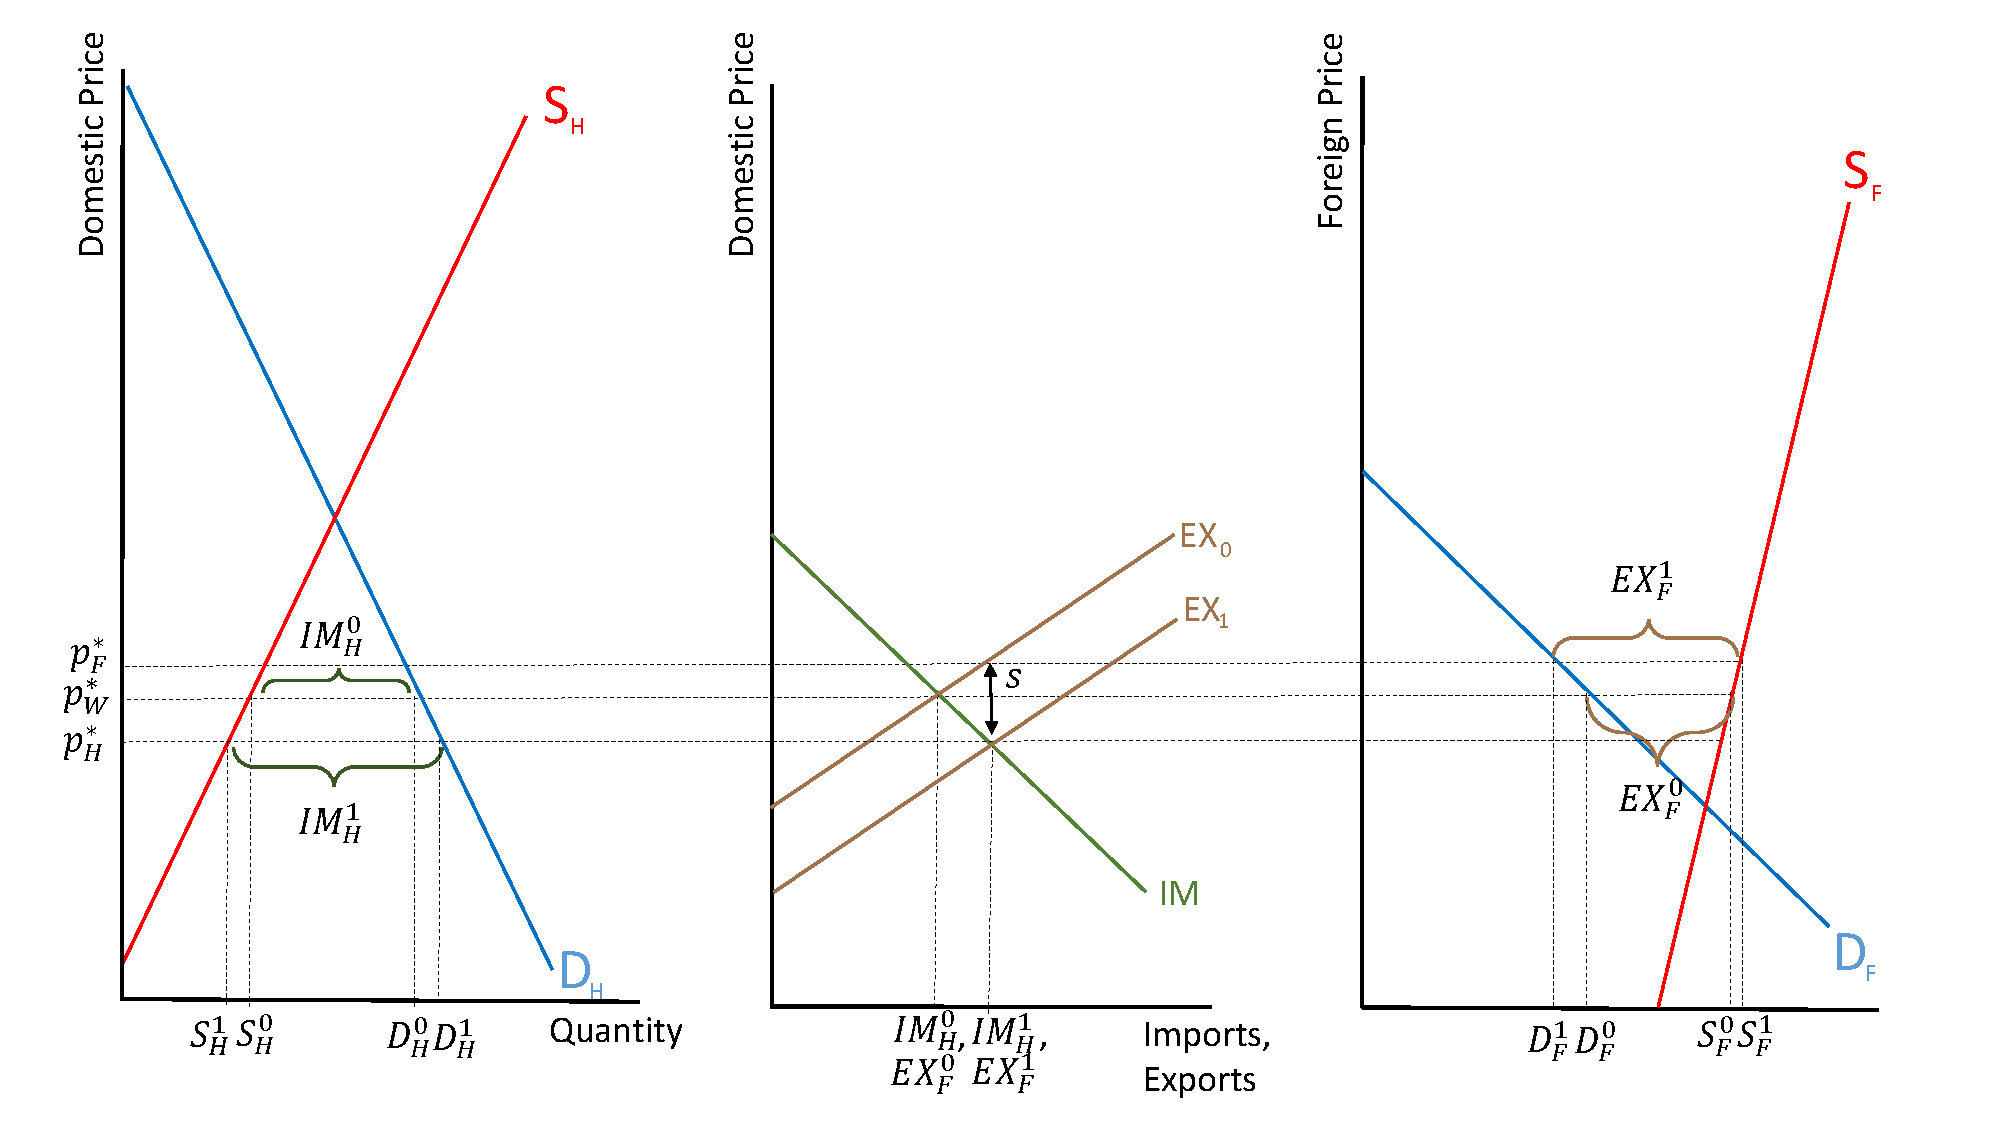
\includegraphics[scale=0.3]{SL_23.pdf}
	
\end{frame}


\begin{frame}
	\frametitle{Export Subsidies and Foreign Welfare: Surplus pre-subsidy}
	
	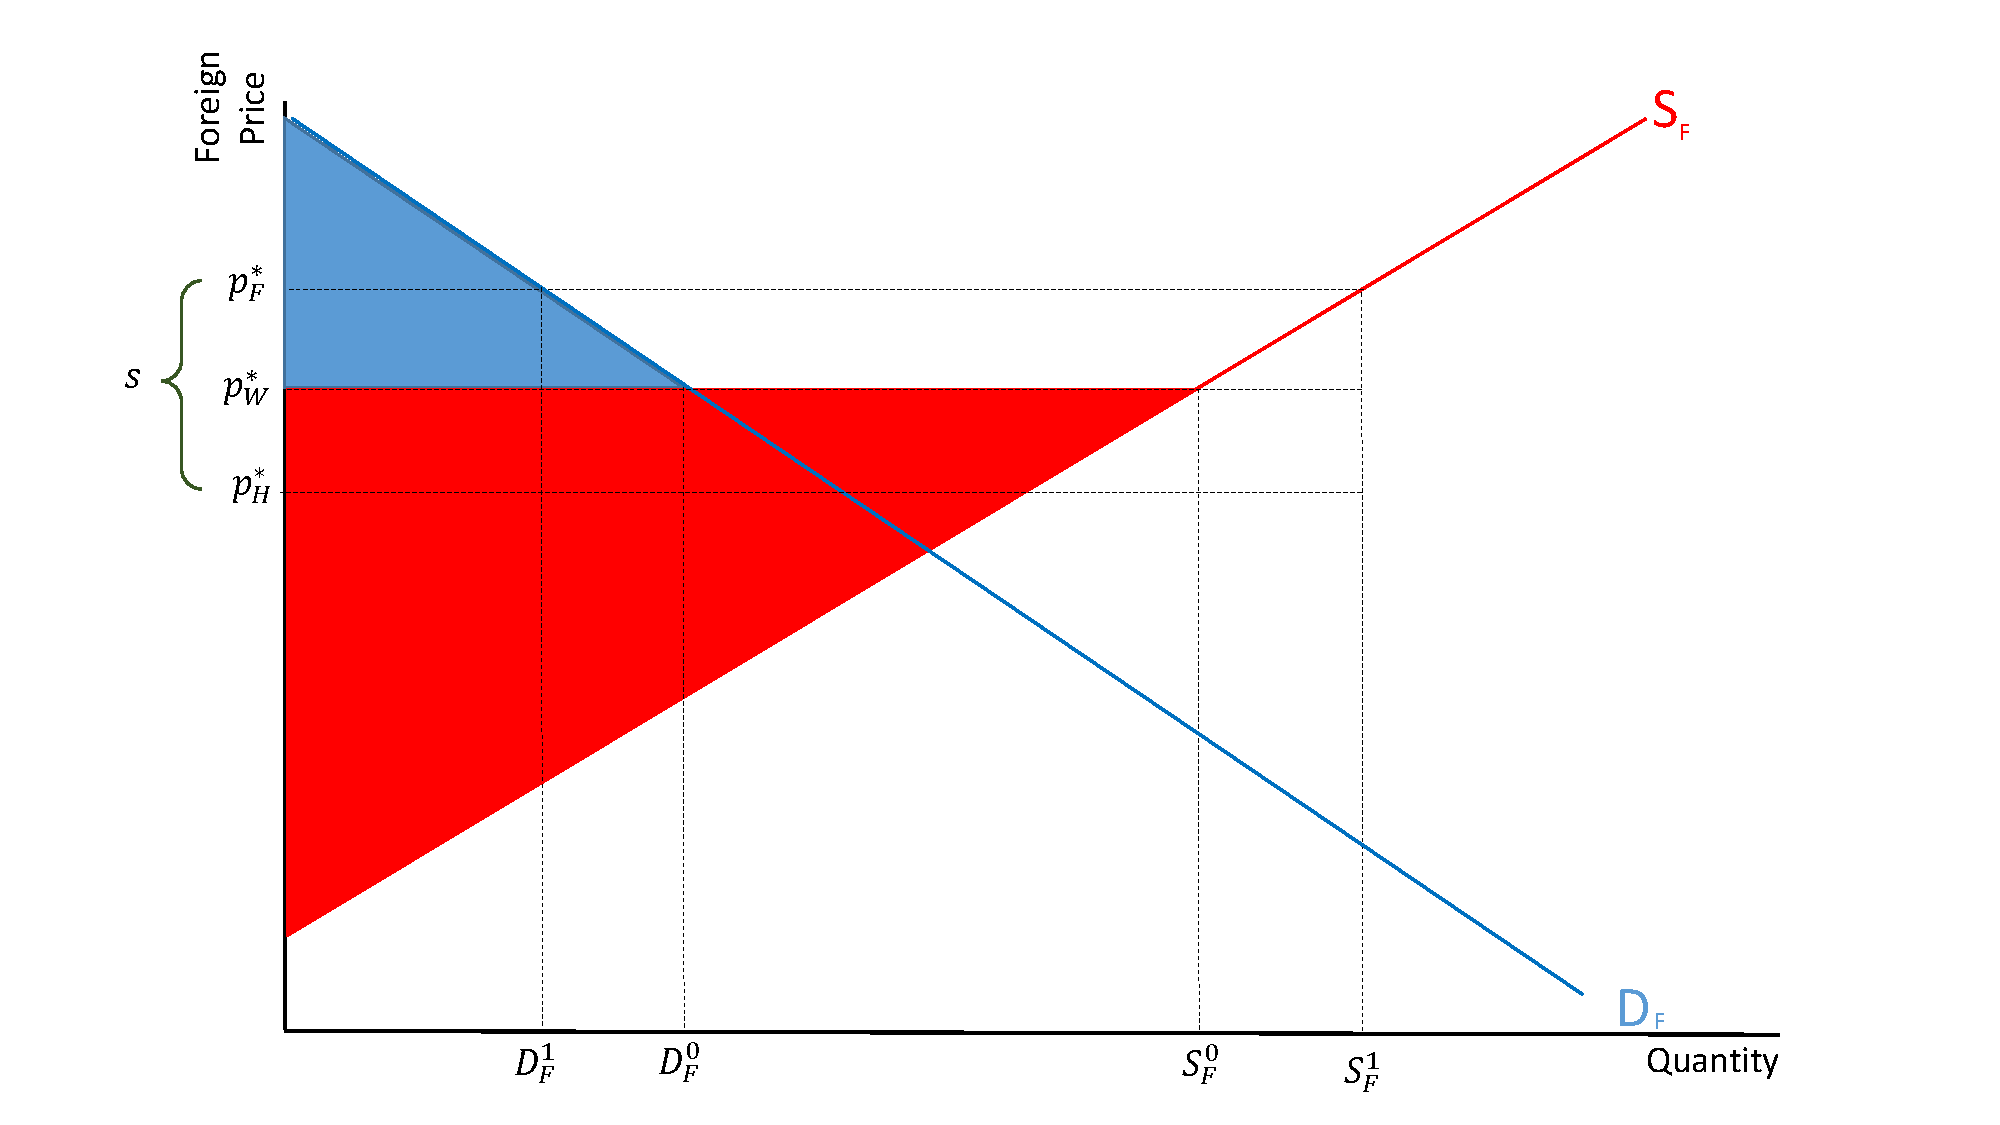
\includegraphics[scale=0.3]{SL_24.pdf}
	
\end{frame}

\begin{frame}
	\frametitle{Export Subsidies and Foreign Welfare: Surplus post-subsidy}
	
	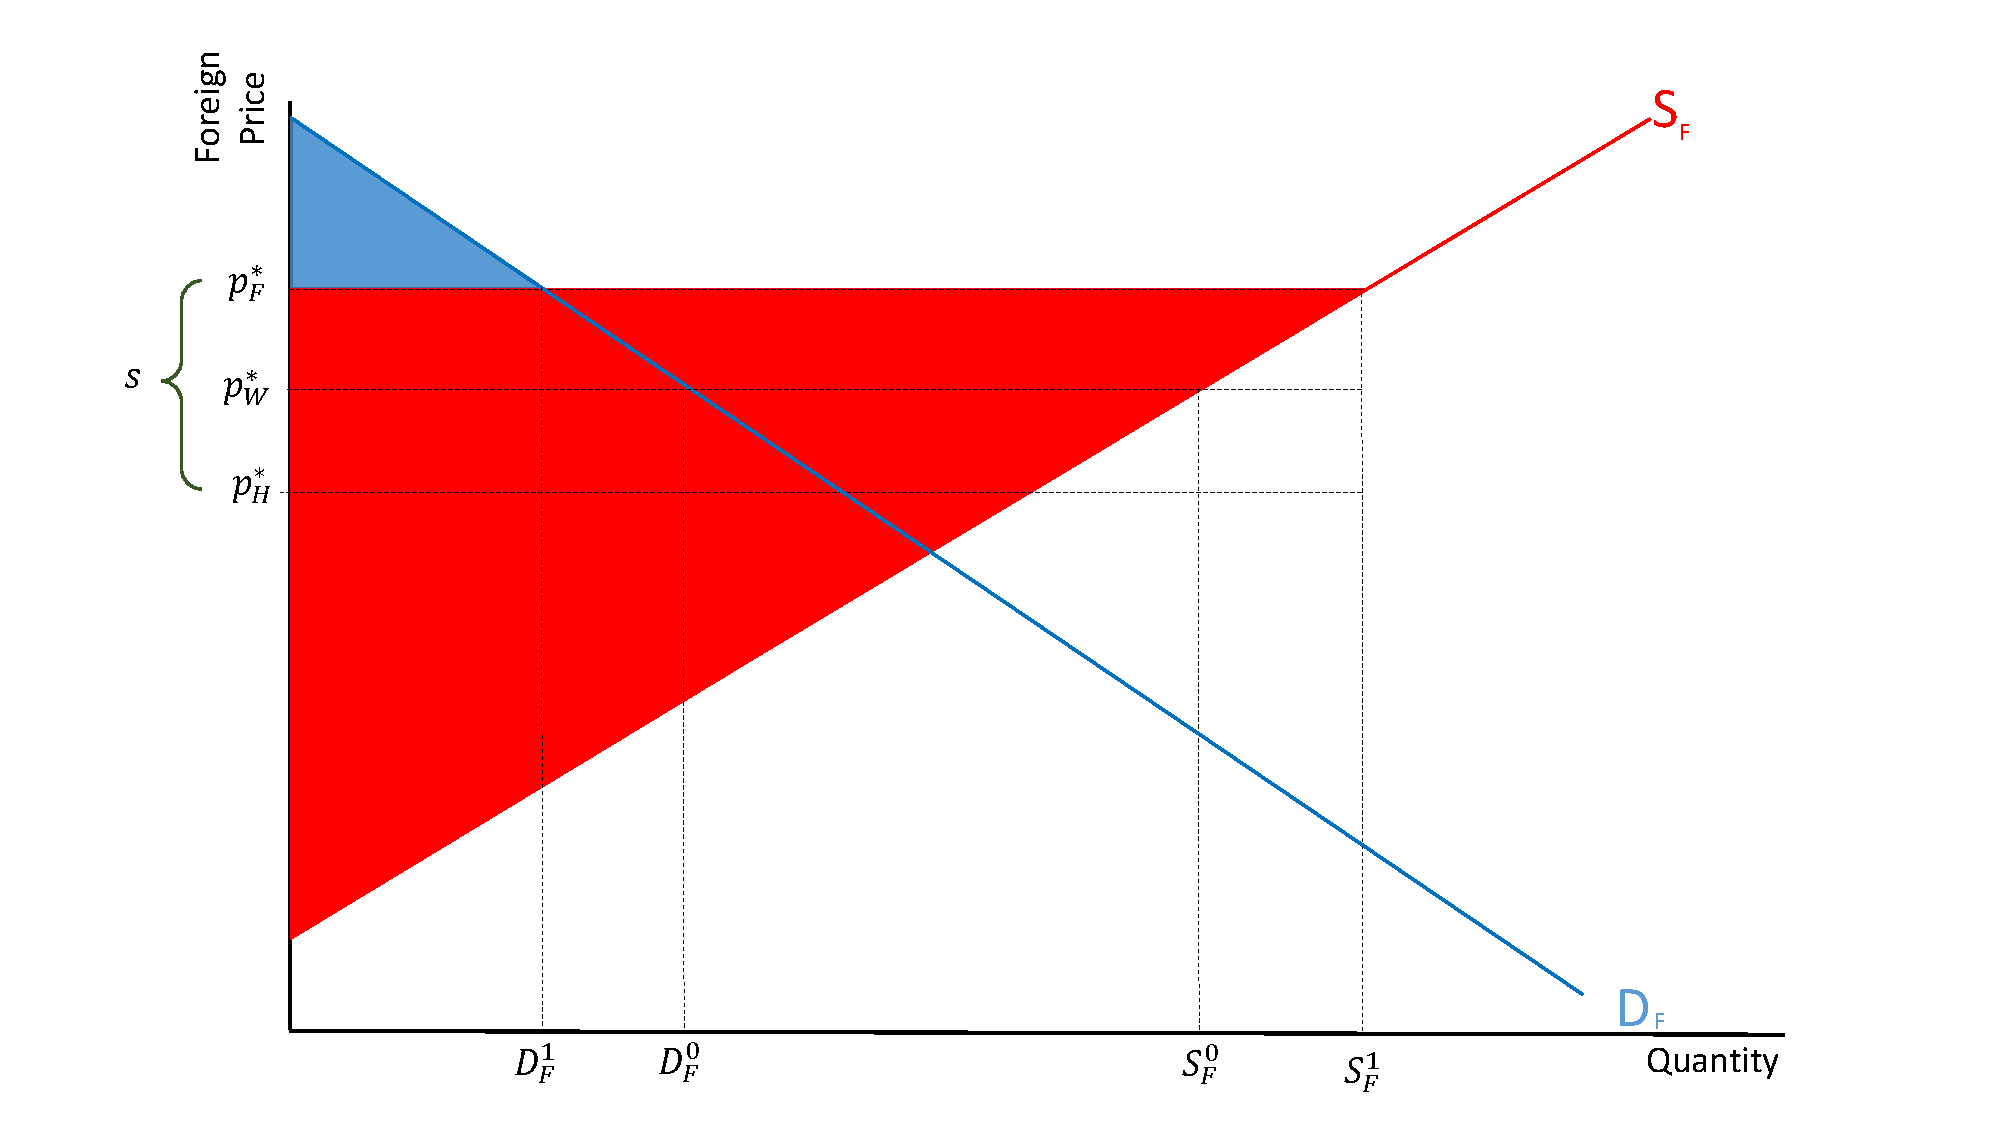
\includegraphics[scale=0.3]{SL_25.pdf}
	
	
	...However, recall that the subsidy must be paid by someone!
	
\end{frame}

\begin{frame}
	\frametitle{Export Subsidies and Foreign Welfare:  Cost of subsidy}
	
	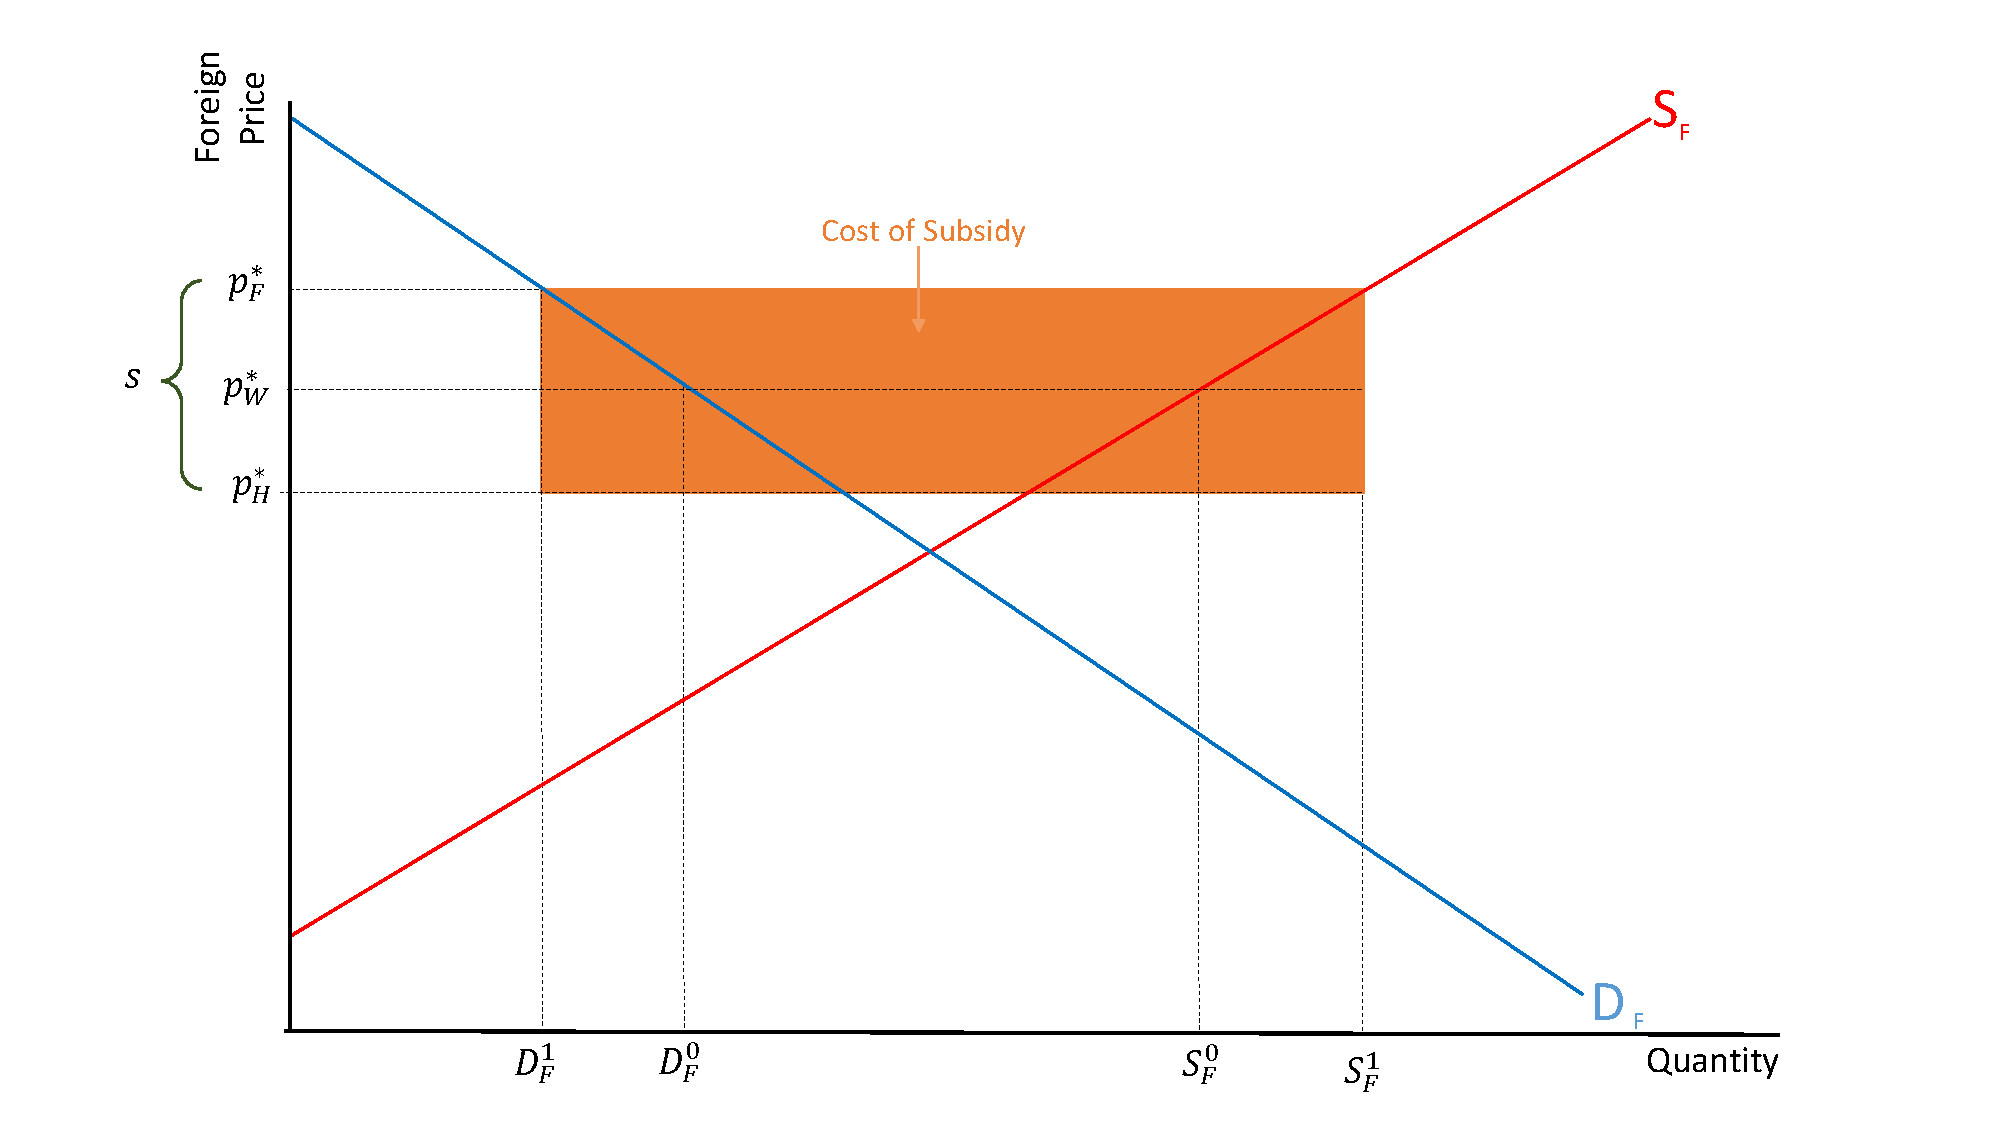
\includegraphics[scale=0.3]{SL_26.pdf}
	
\end{frame}

\begin{frame}
	\frametitle{Export Subsidies and Foreign Welfare:  Change in surplus}
	
	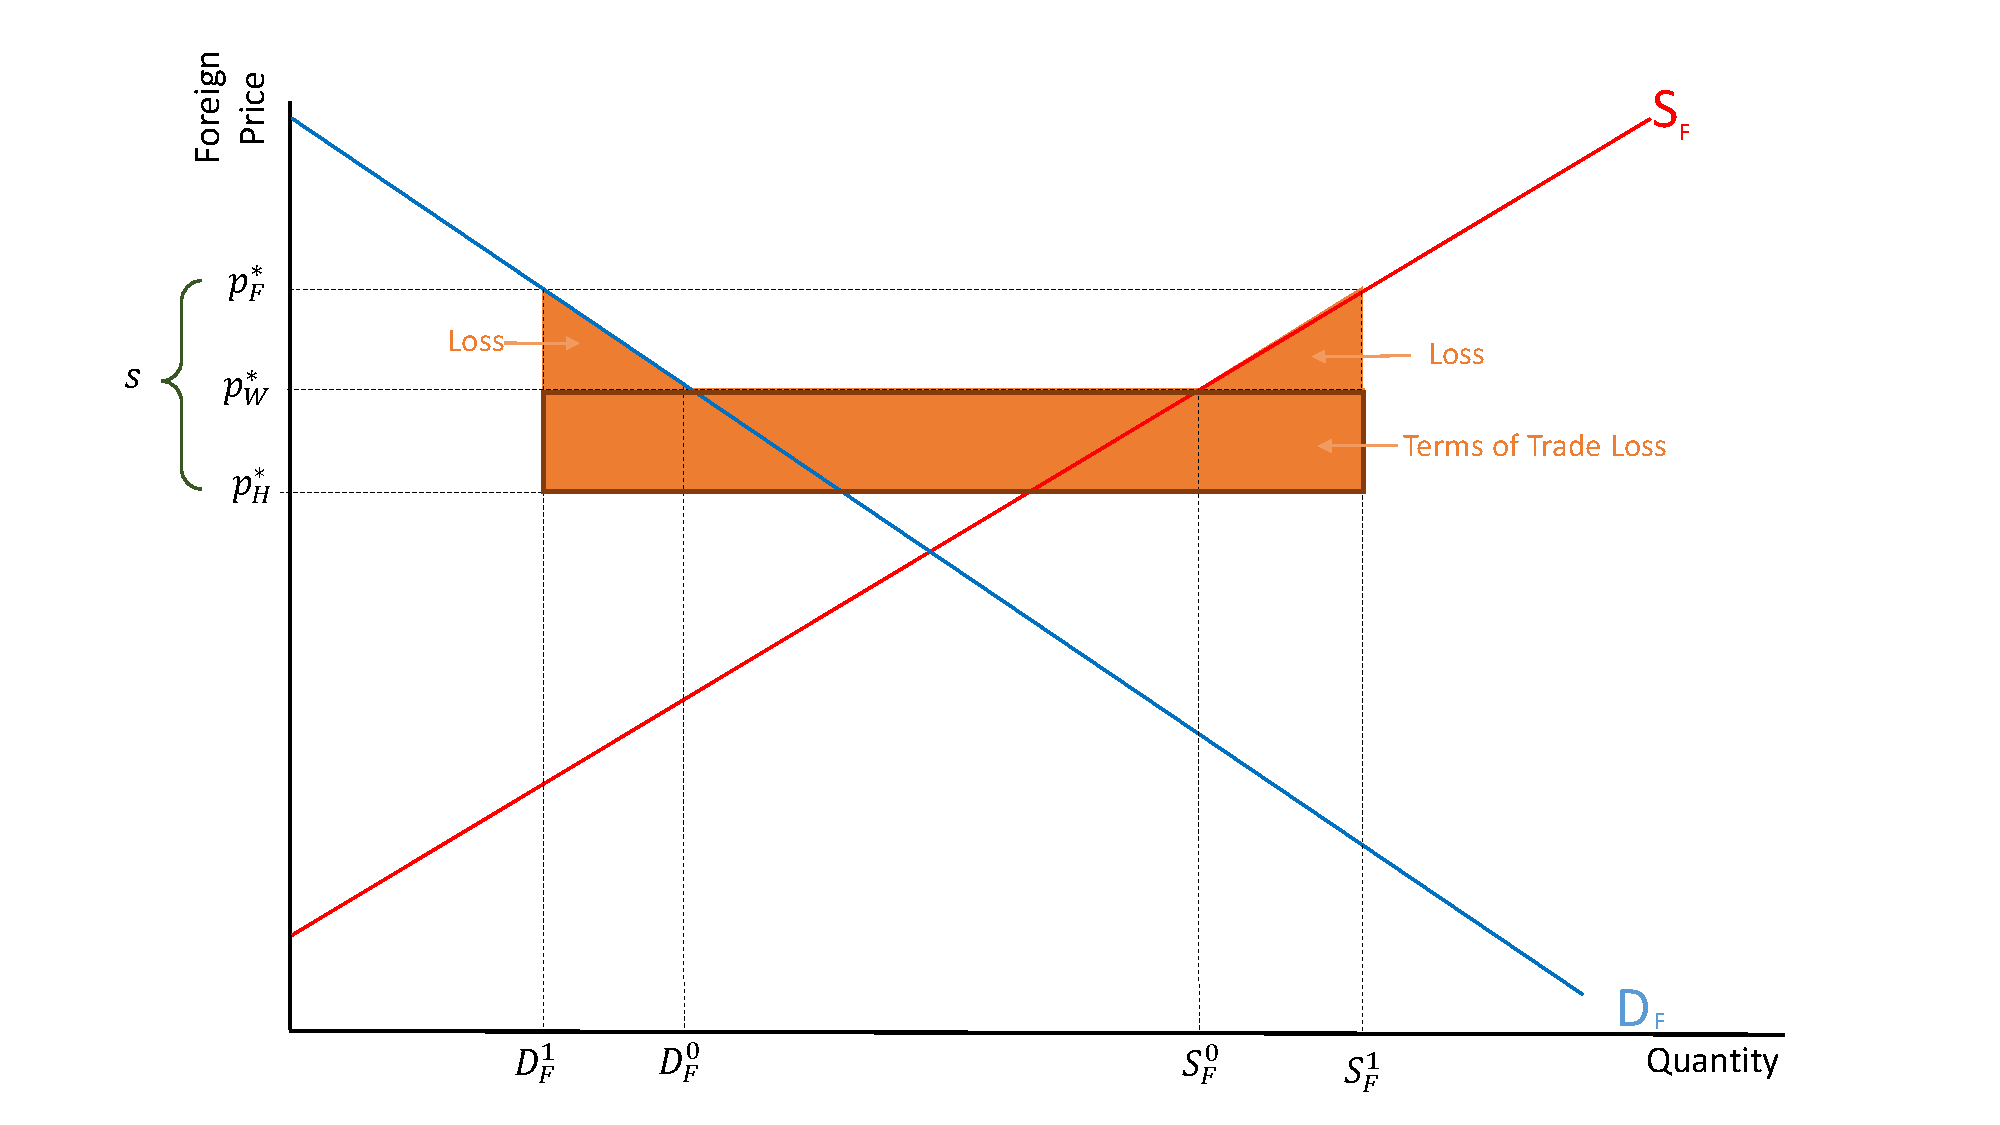
\includegraphics[scale=0.3]{SL_27.pdf}
	
\end{frame}

\begin{frame}
	\frametitle{Export Subsidies:  Summary}
	
	\begin{itemize}
		\item Foreign exports and Home imports rise.
		\item Export subsidies cost the Foreign government money \emph{and decrease} Foreign's terms of trade.
		\begin{itemize}
			\item The Foreign price of the good rises, while the Home price falls.
			\item Leads to an extra welfare cost for the Foreign country.
		\end{itemize}
		\item In general export subsidies do not benefit the exporting country. 
		\begin{itemize}
			\item May be used to achieve distributional goals. 
			\begin{itemize}
				\item Eg. European Common Agricultural Policy.
			\end{itemize} 
		\end{itemize}
		
	\end{itemize}
	
\end{frame}

\subsection{Quotas}
\begin{frame}
	\frametitle{Quotas}
	\textbf{Import Quotas}: A government imposed restriction on the quantity of some good that may imported. 
	\begin{itemize}
		\item Usually enforced issuing import licenses to some limited number of firms.	
		\begin{itemize}
			\item License allows them to import at most some limited quantity of a good. 
		\end{itemize}
		\item Common misconception: Since we are only limiting the quantity of imports, no impact on prices.
		\begin{itemize}
			\item \emph{A (binding) import quota always raises the domestic price of the imported good}
			\begin{itemize}
				\item If import quota binding, then Demand $>$ Supply, domestic prices will be bid up!
			\end{itemize}
		\end{itemize}
	\end{itemize}
	
	
\end{frame}


\begin{frame}
	\frametitle{Quotas: Small Open Economy}
	
	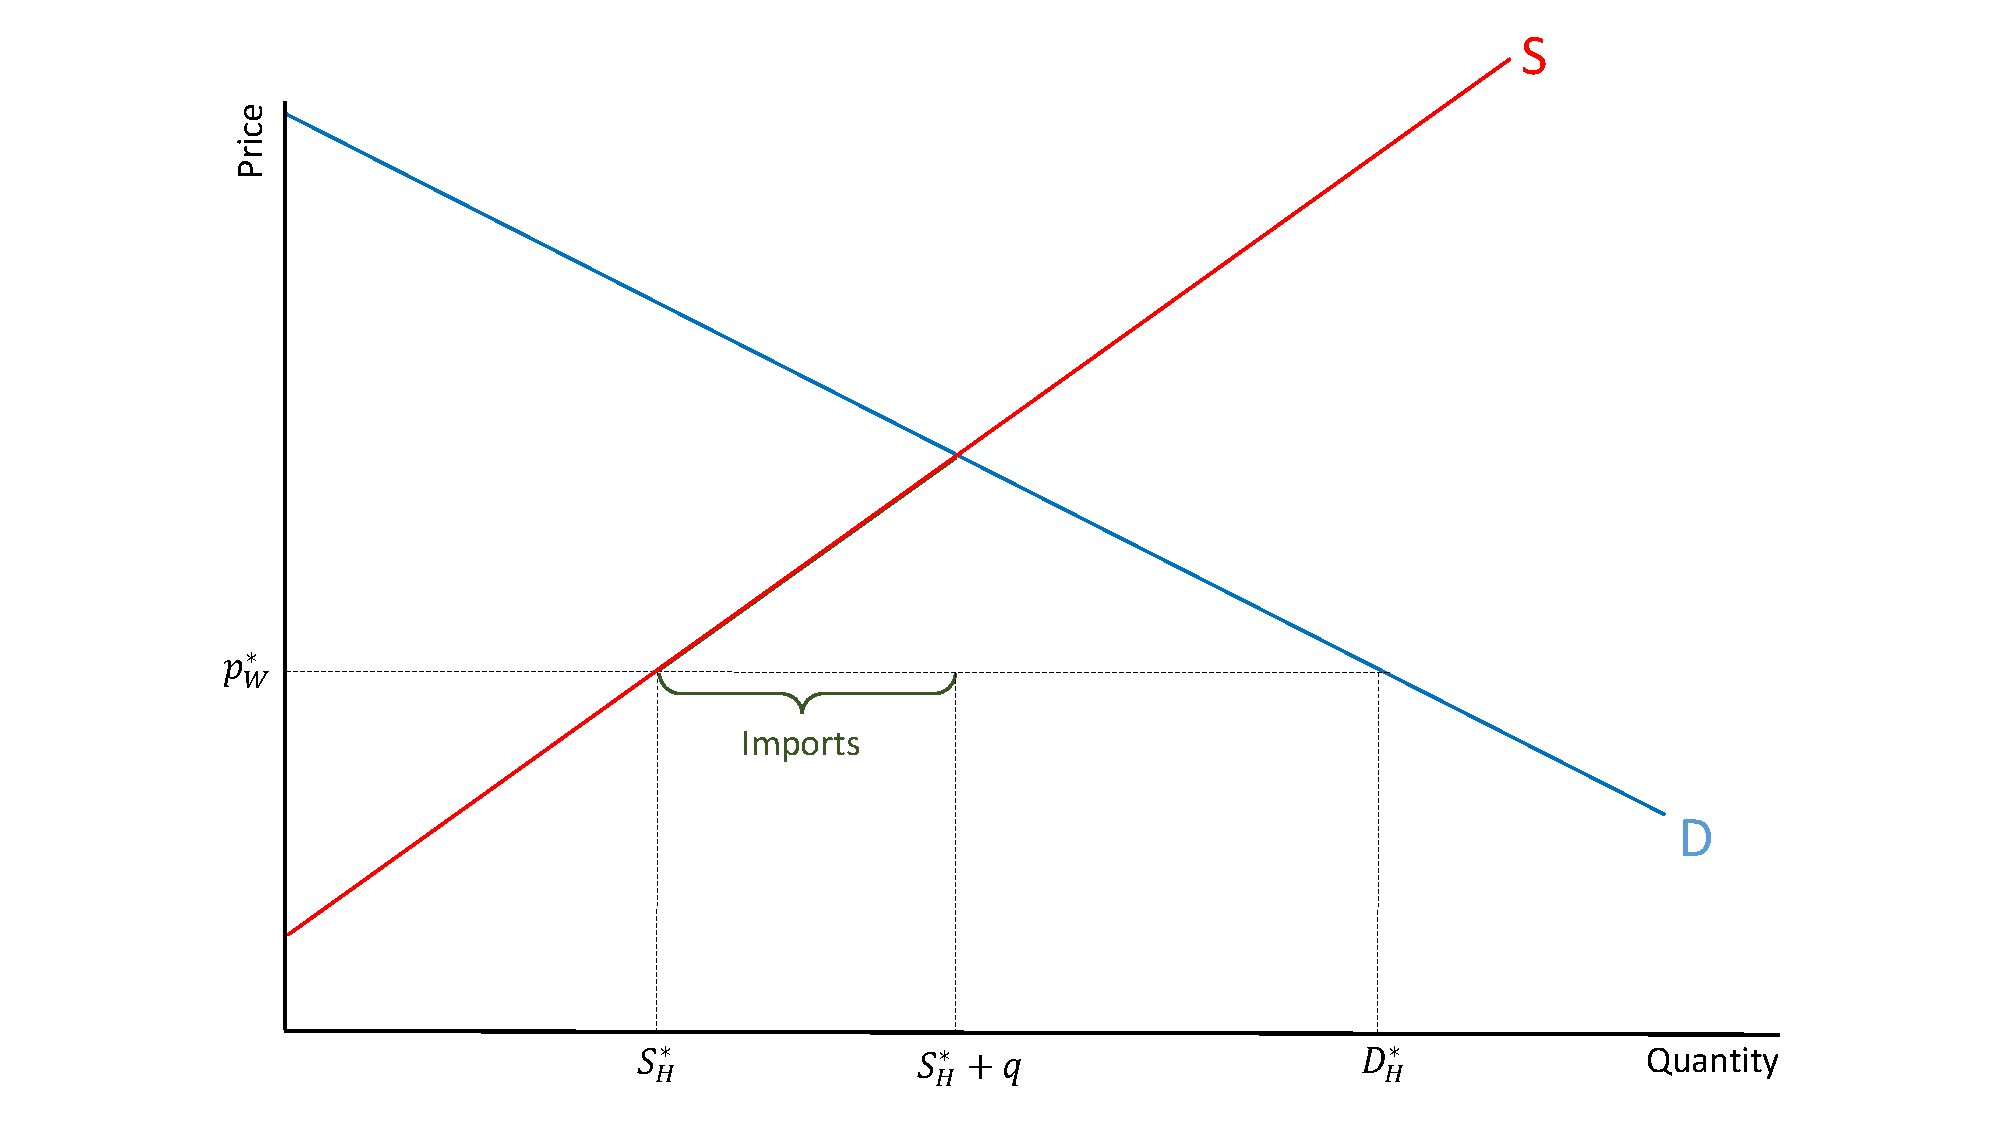
\includegraphics[scale=0.3]{SL_16.pdf}
	
\end{frame}

\begin{frame}
	\frametitle{Quotas: Small Open Economy}
	
	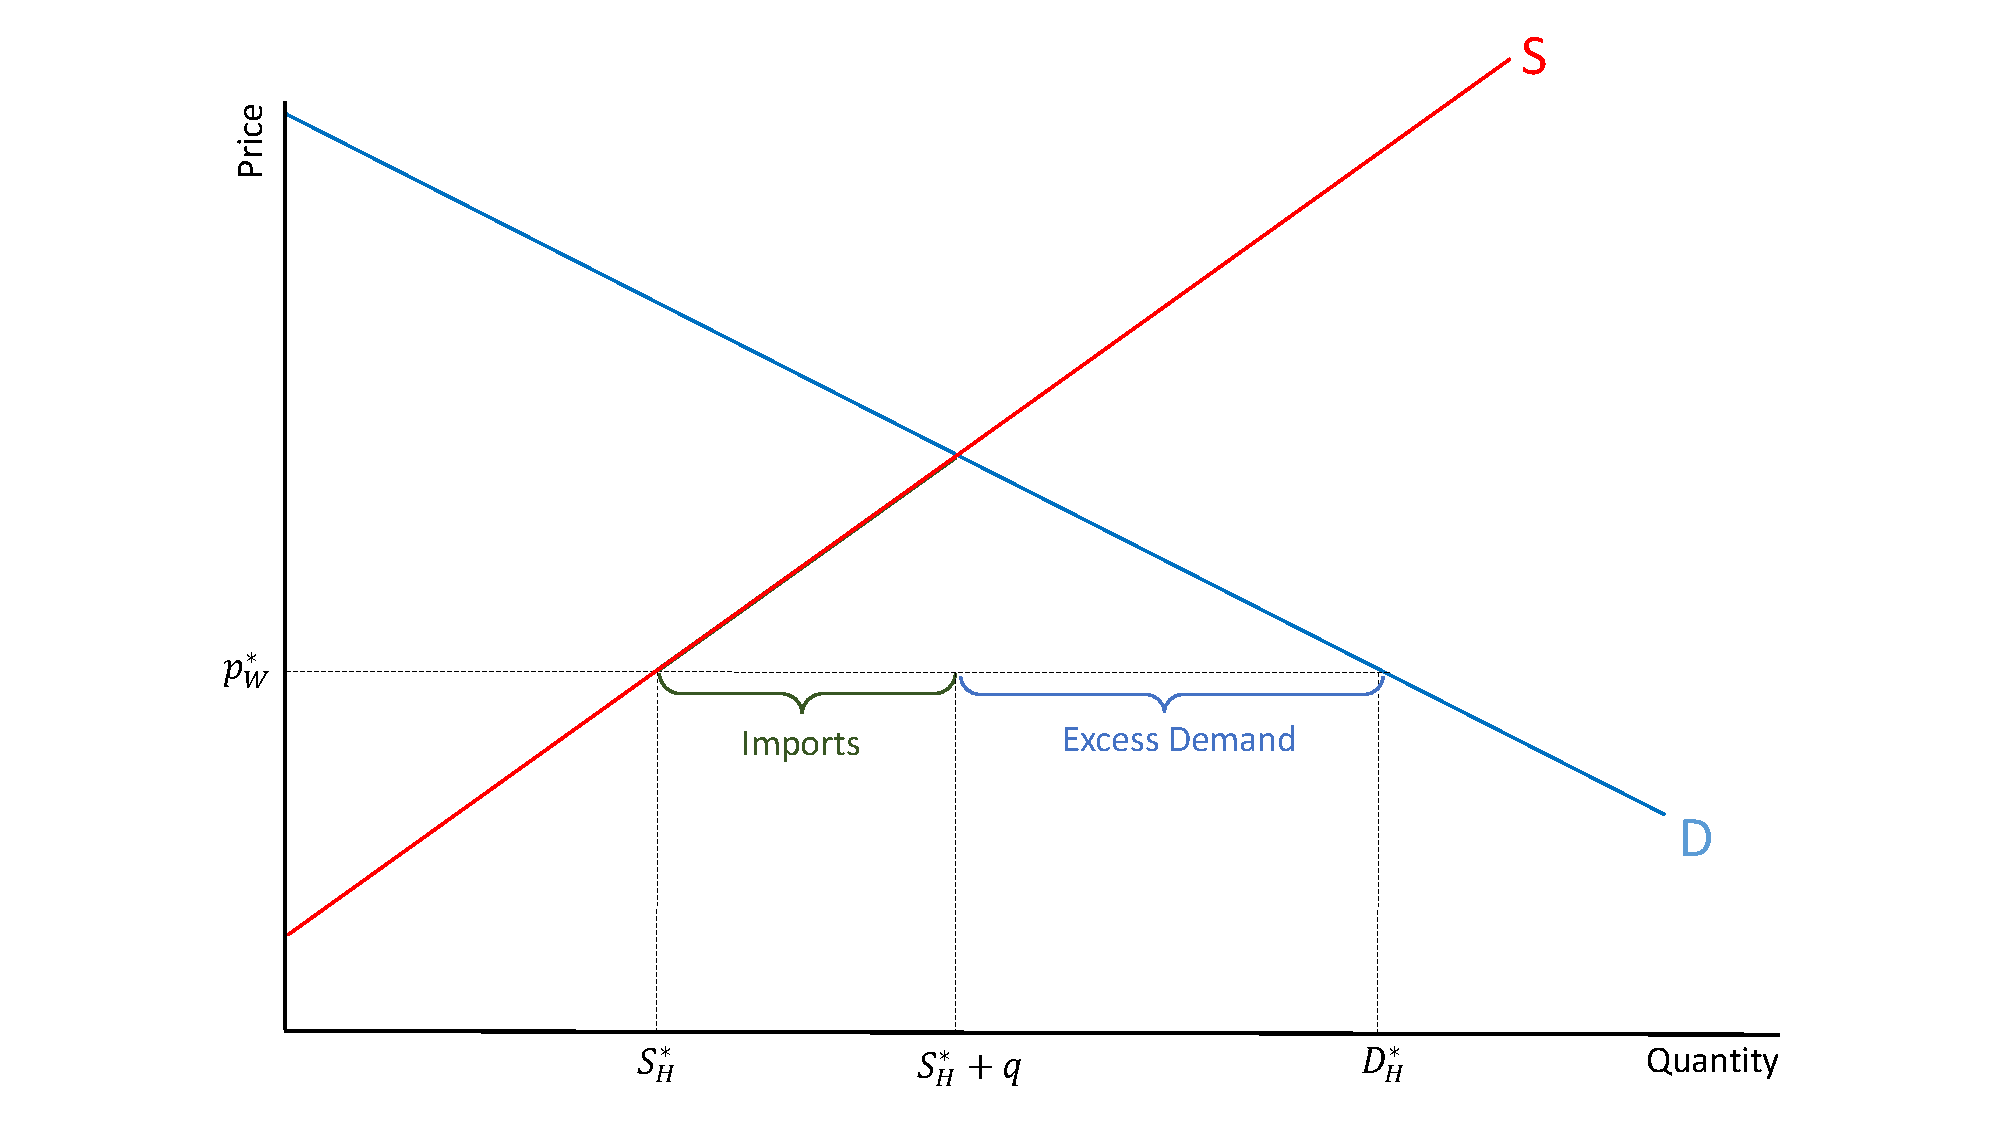
\includegraphics[scale=0.3]{SL_17.pdf}
	
\end{frame}

\begin{frame}
	\frametitle{Quotas: Small Open Economy}
	
	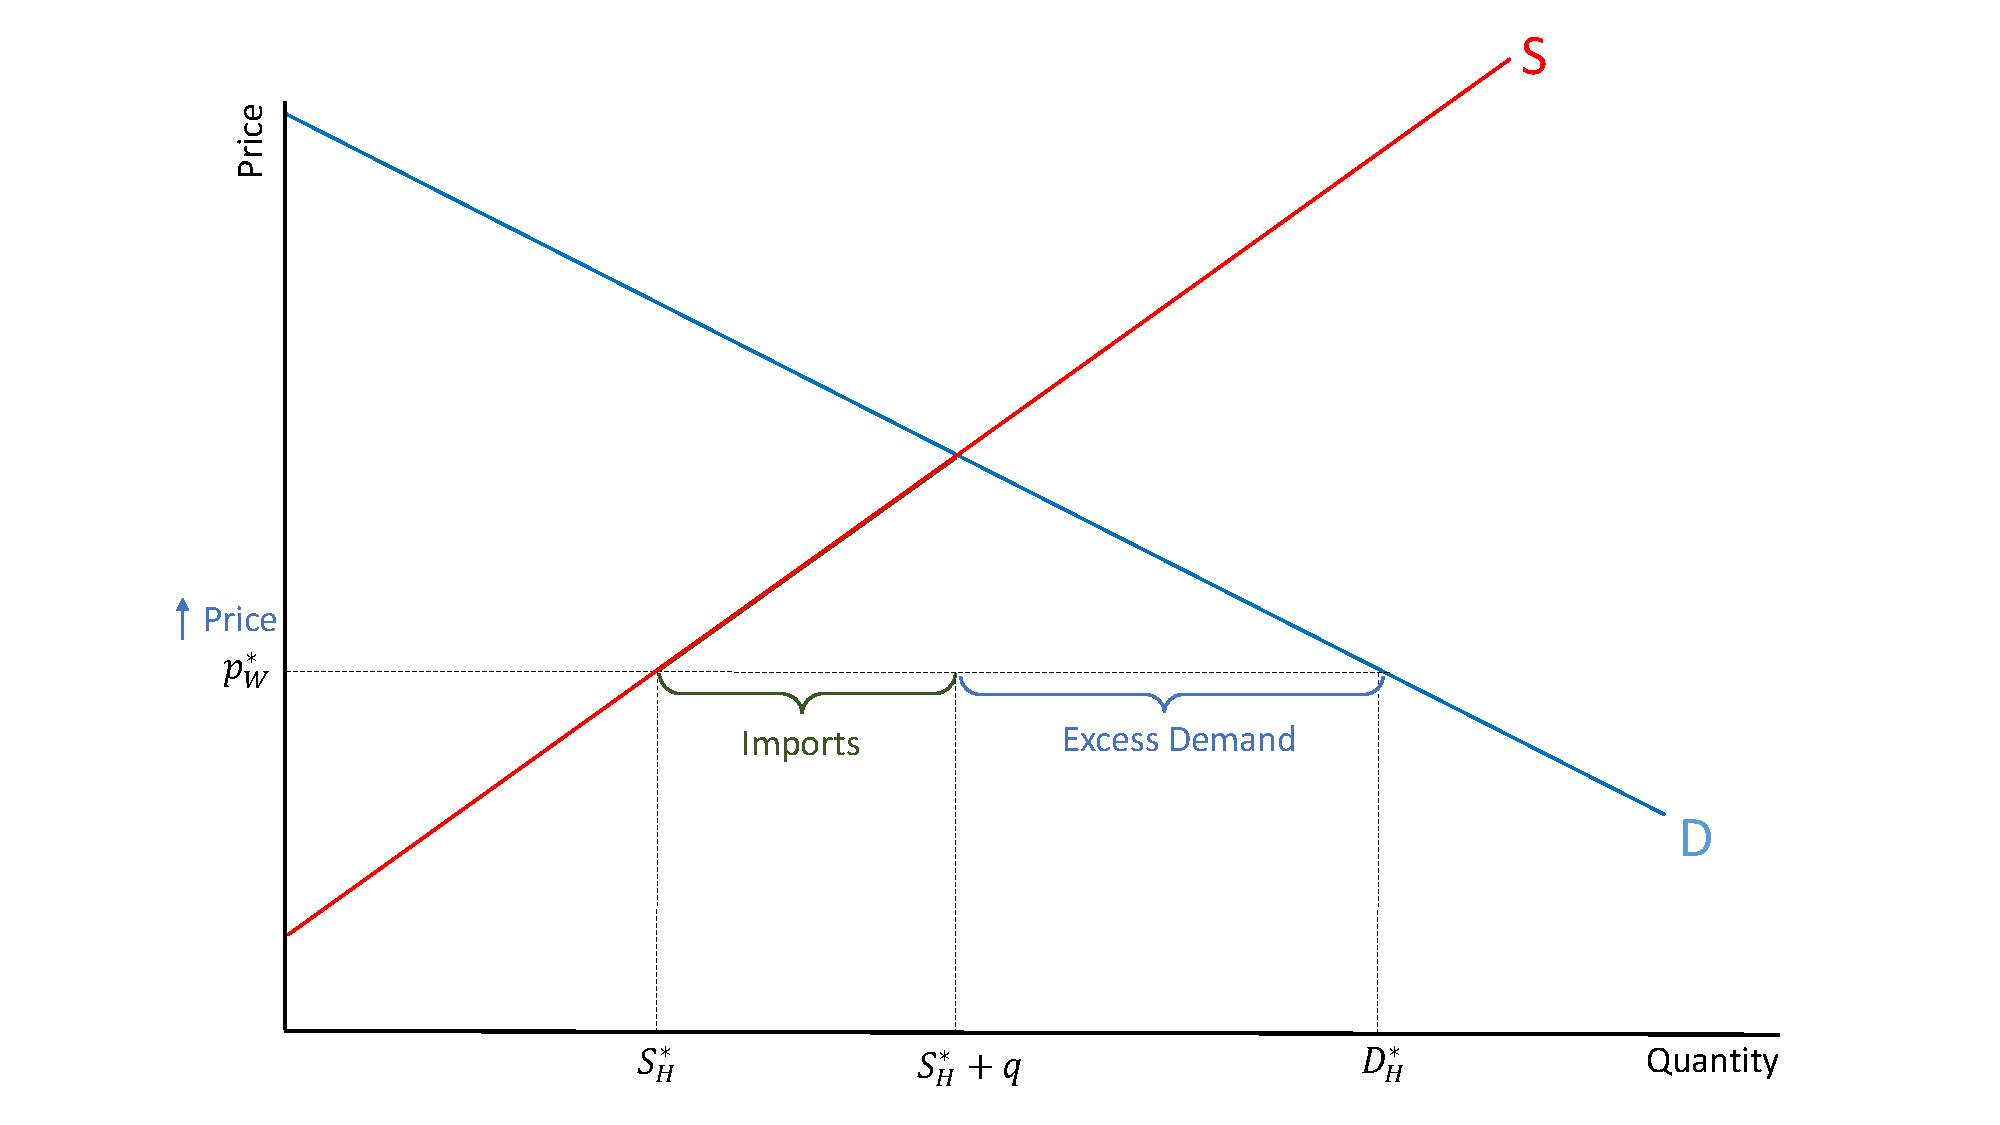
\includegraphics[scale=0.3]{SL_18.pdf}
	
\end{frame}

\begin{frame}
	\frametitle{Quotas: Small Open Economy}
	
	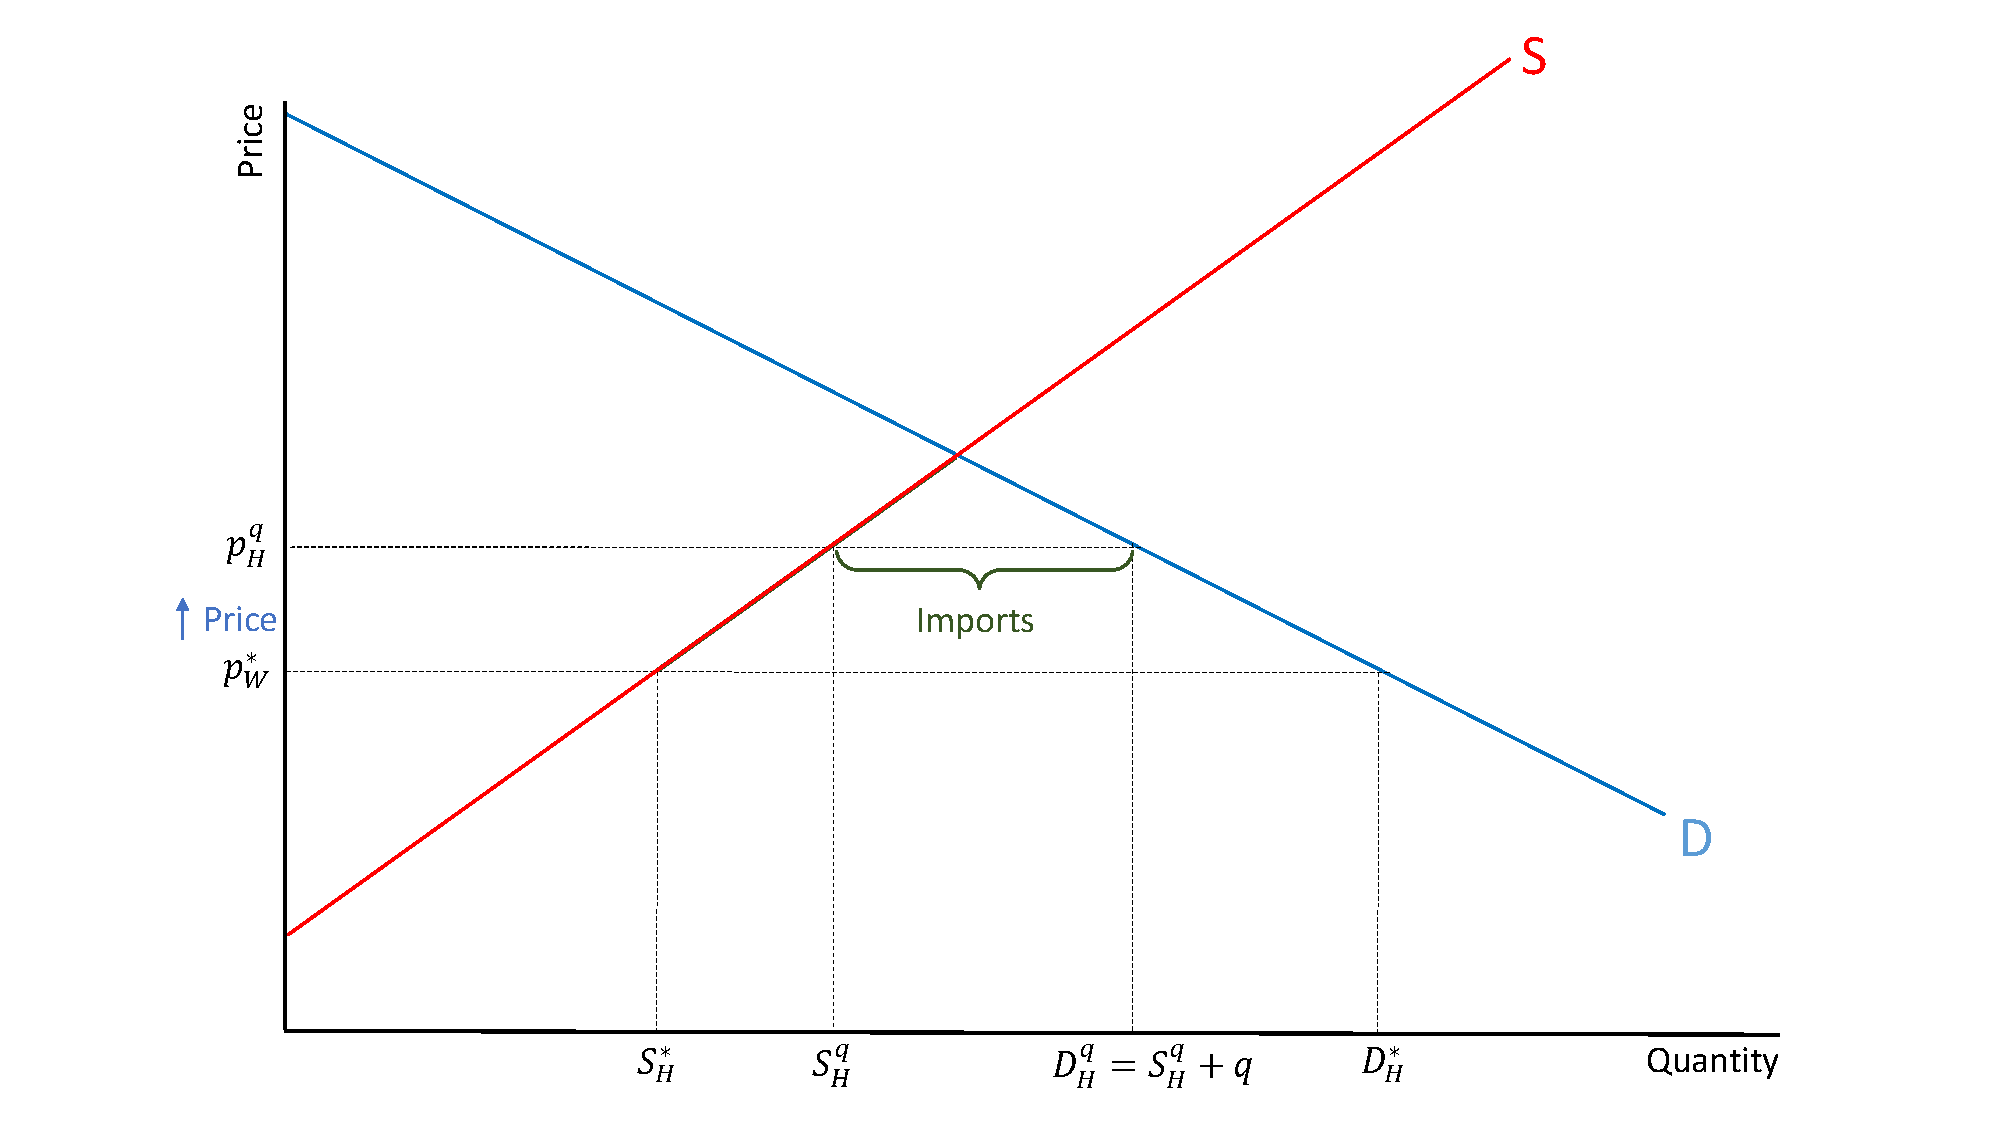
\includegraphics[scale=0.3]{SL_19.pdf}
	
\end{frame}

\begin{frame}
	\frametitle{Quotas and Welfare for SOE: Surplus Pre-Quota}
	
	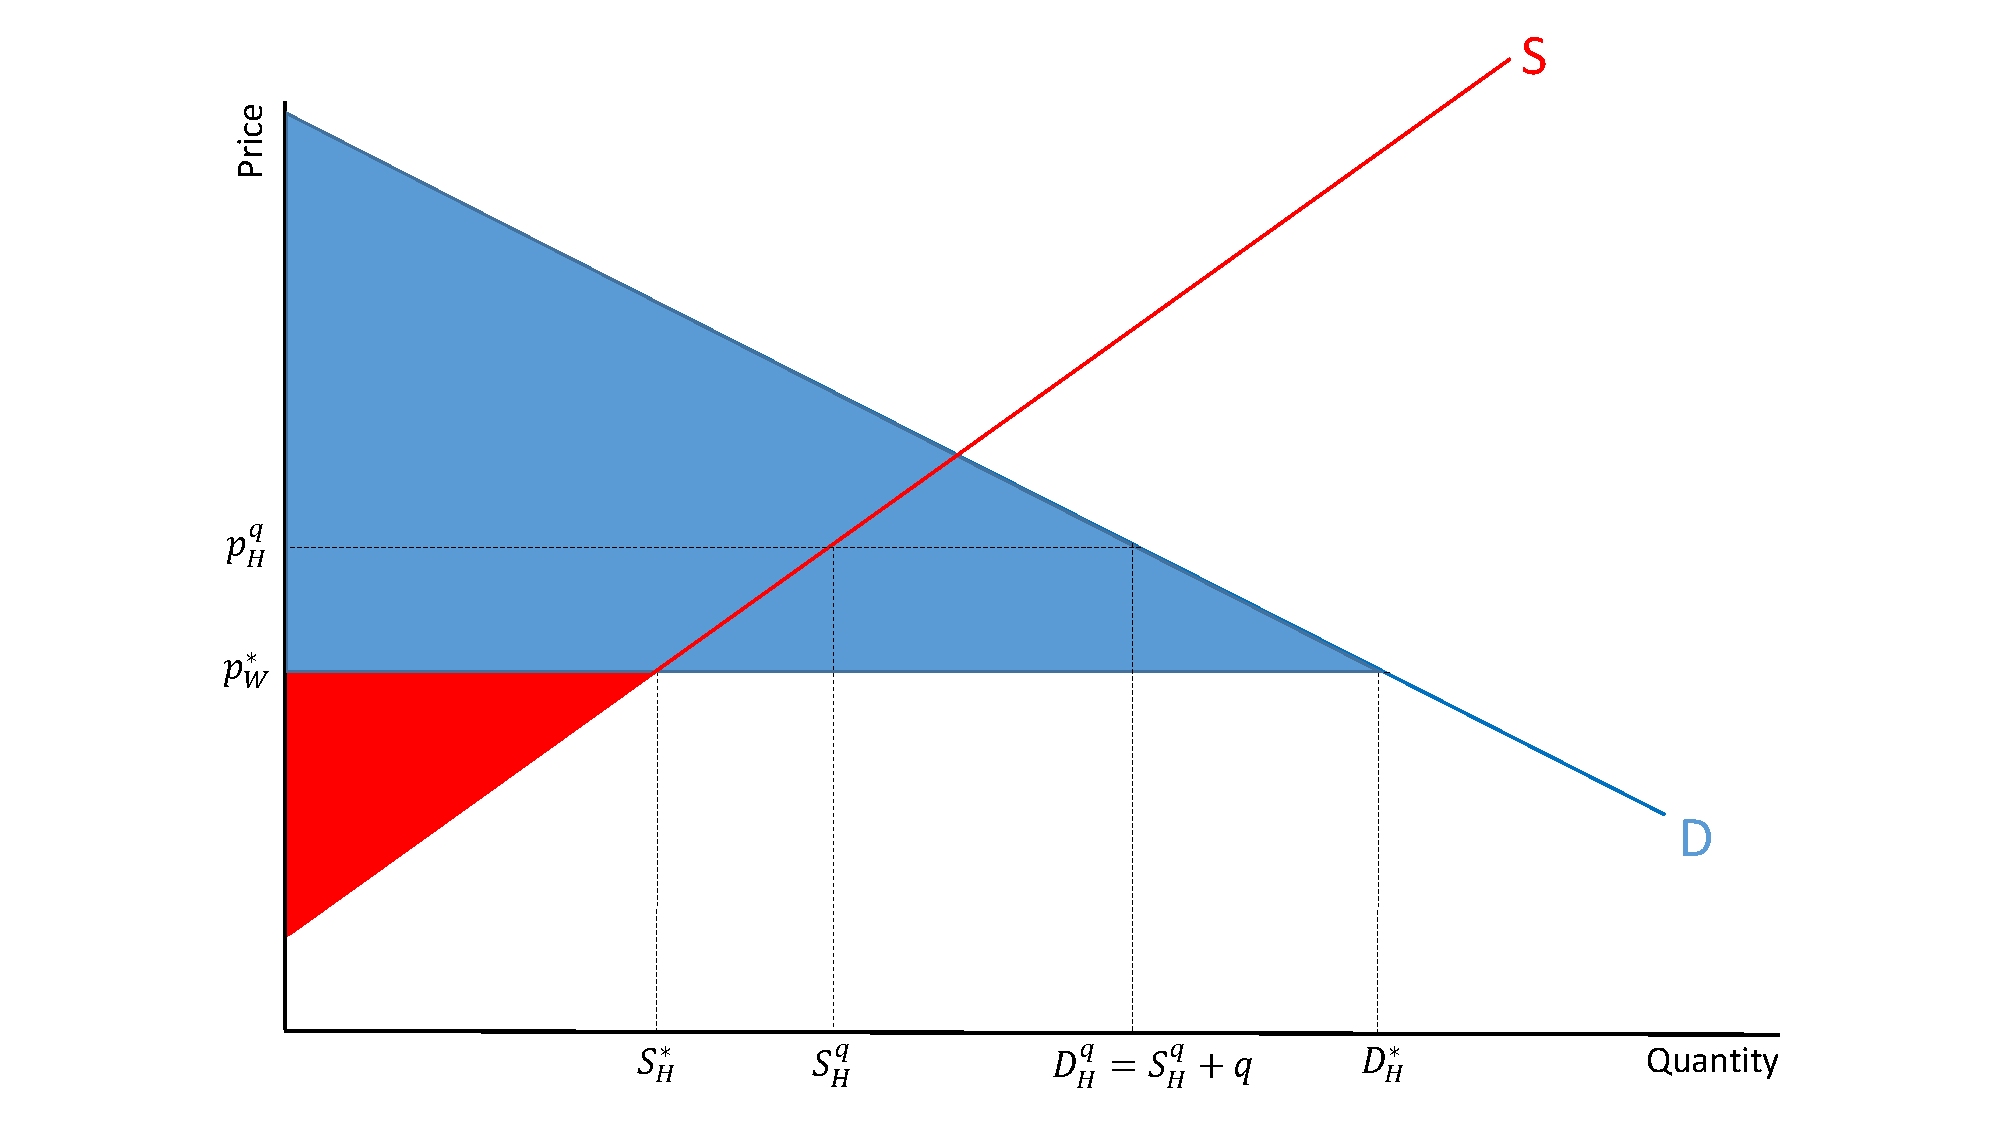
\includegraphics[scale=0.3]{SL_20.pdf}
	
\end{frame}

\begin{frame}
	\frametitle{Quotas and Welfare for SOE: Surplus Post-Quota}
	
	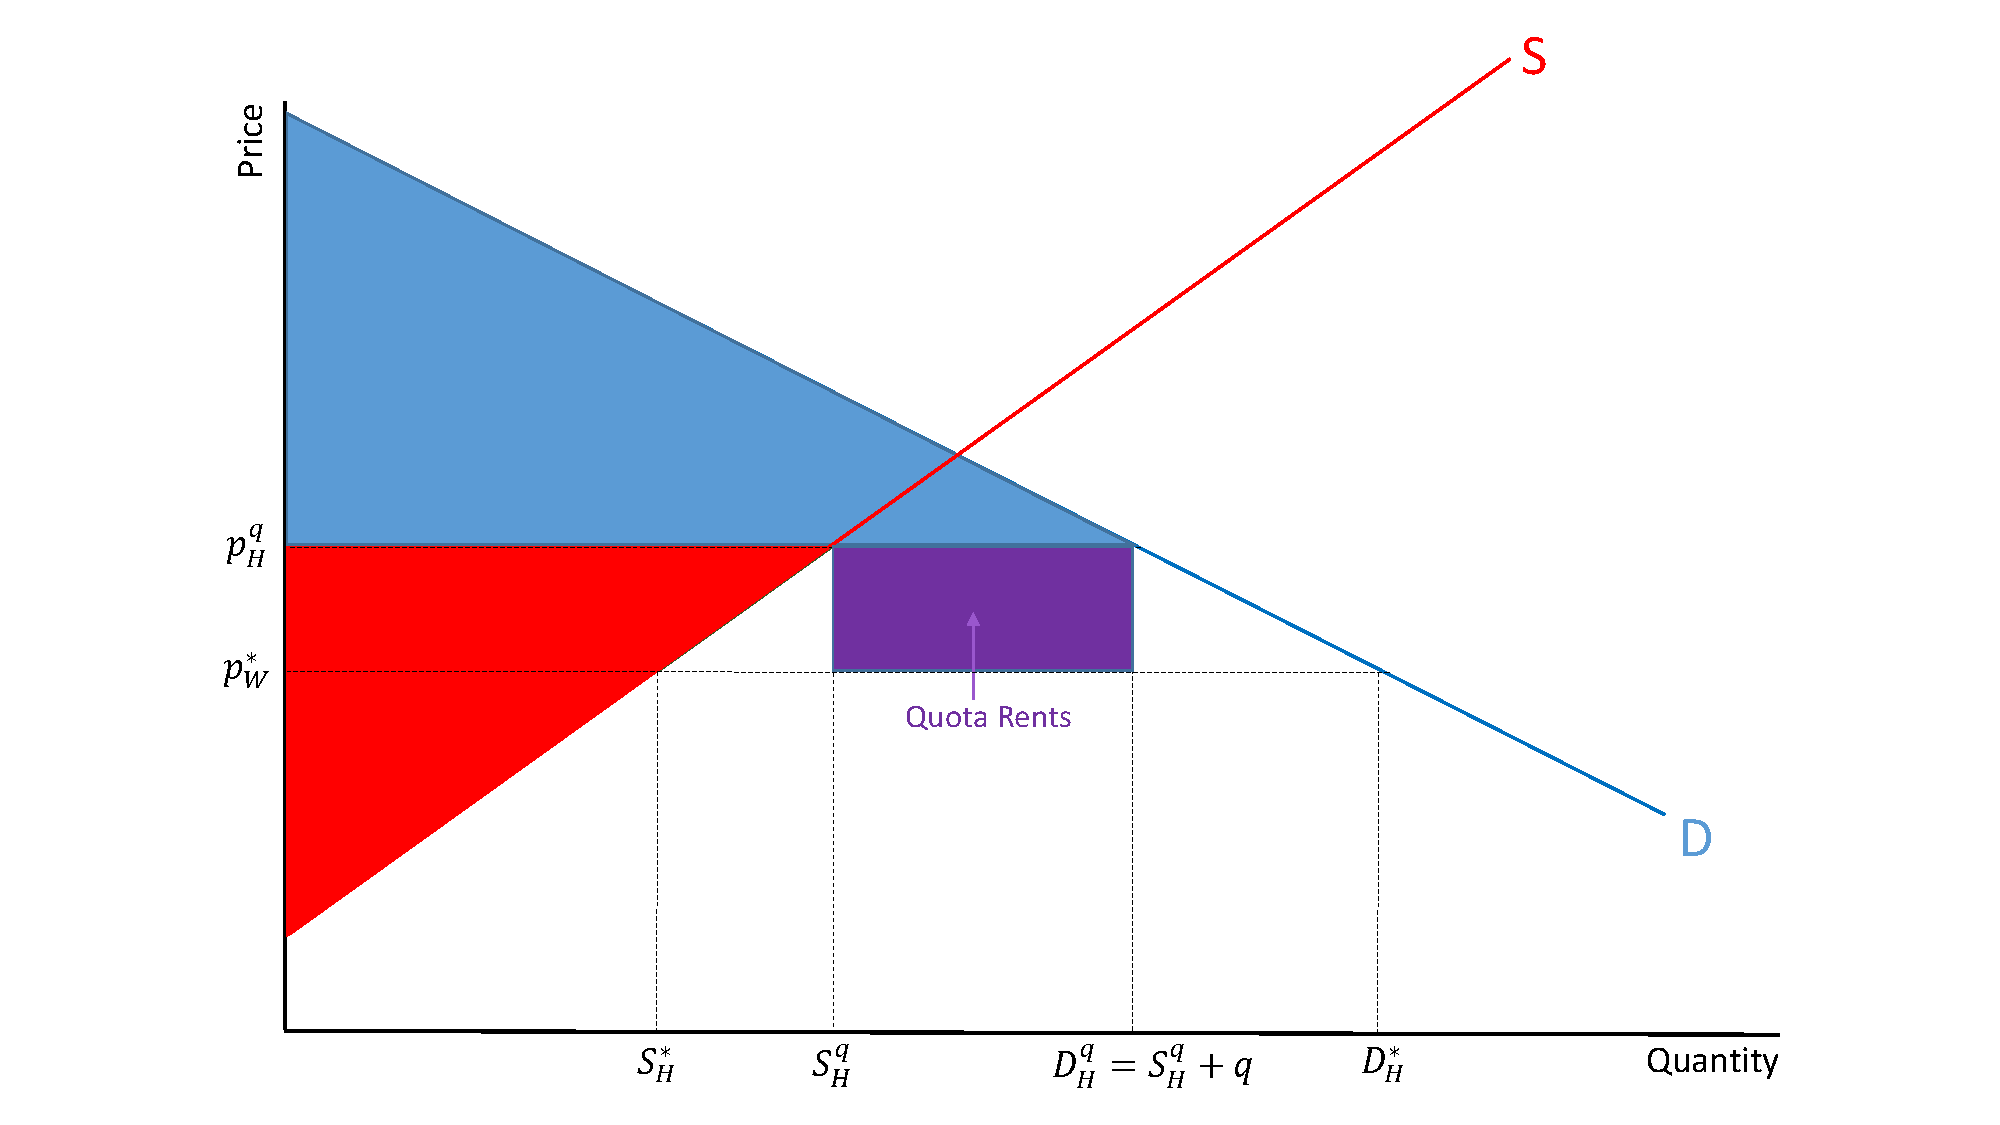
\includegraphics[scale=0.3]{SL_21.pdf}
	
\end{frame}

\begin{frame}
	\frametitle{Quotas and Welfare for SOE: Change in Surplus}
	
	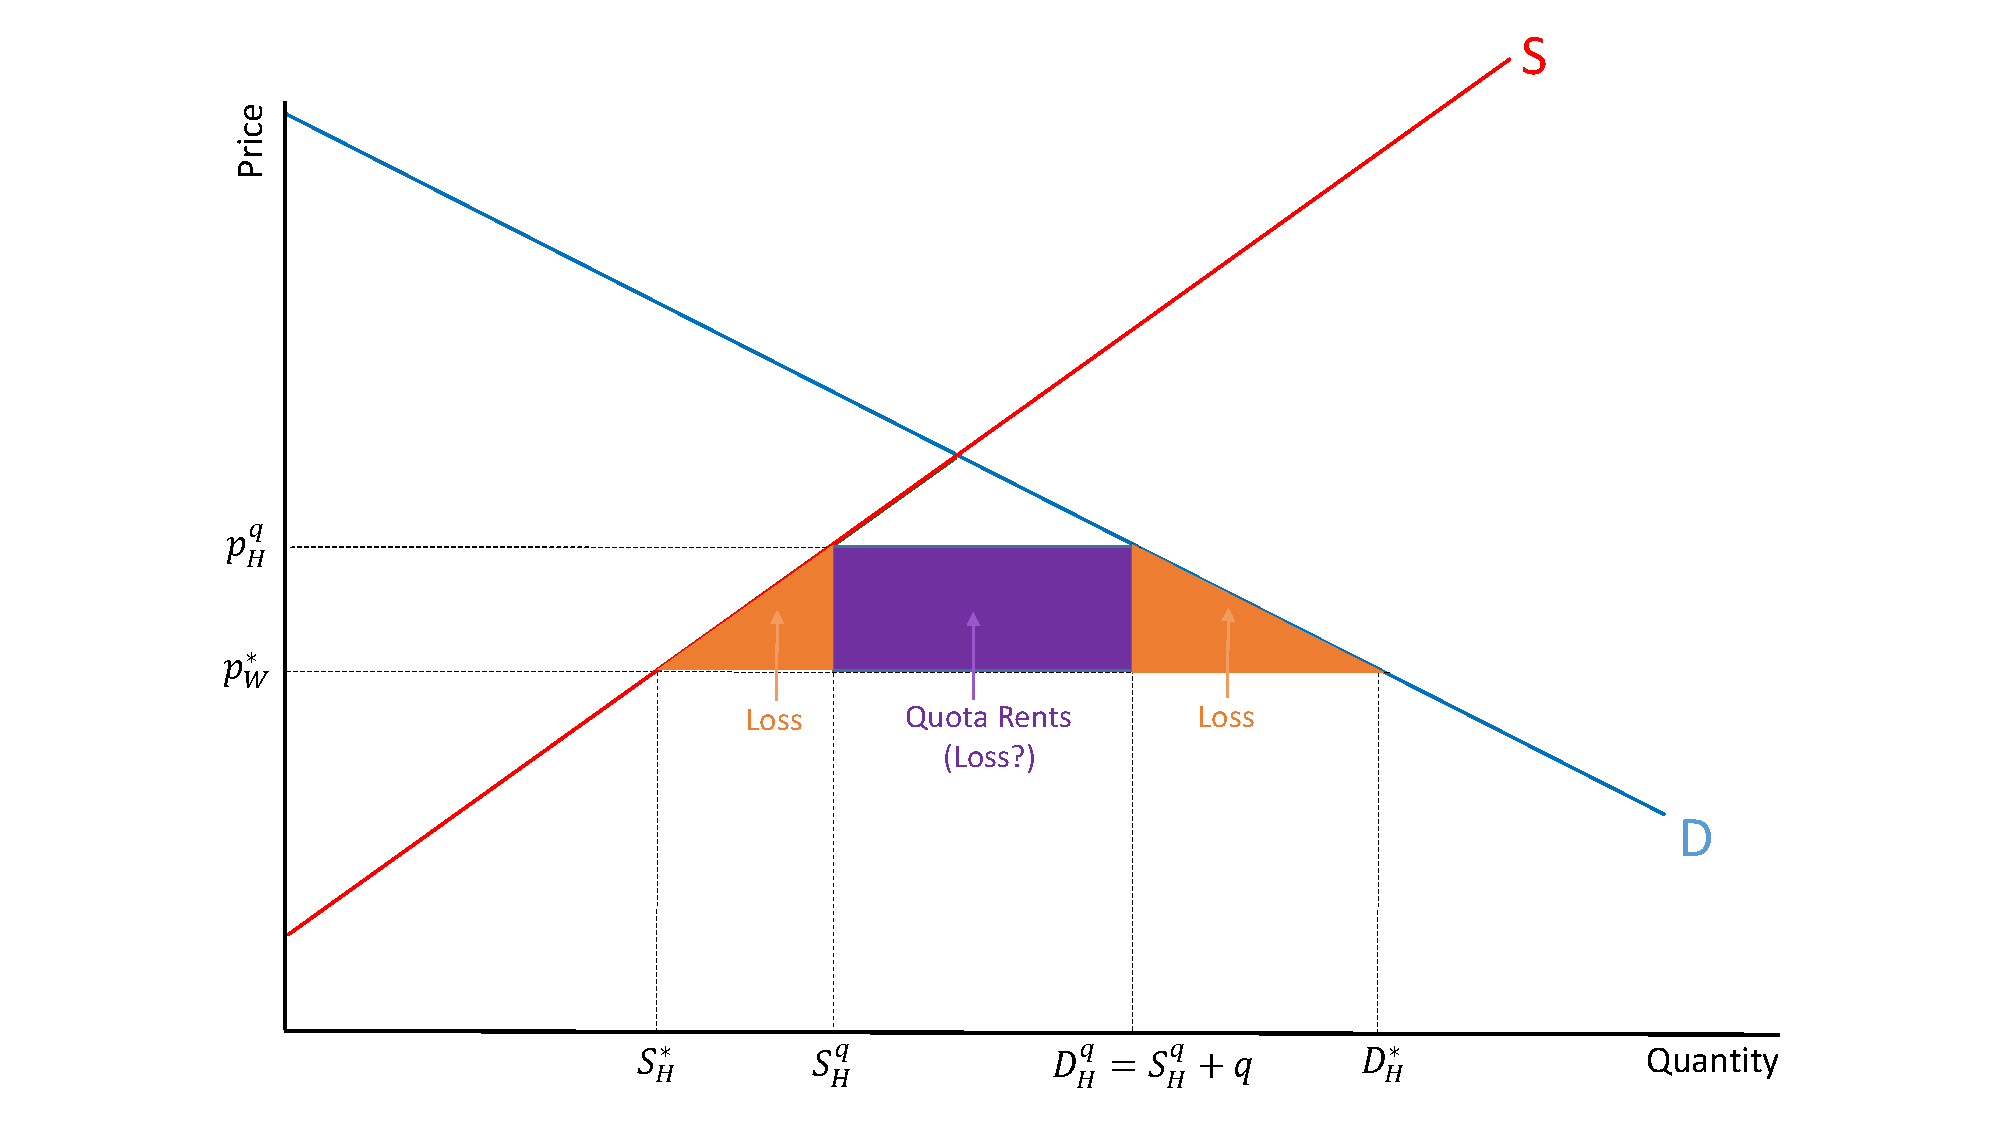
\includegraphics[scale=0.3]{SL_22.pdf}
	
\end{frame}

\begin{frame}
	\frametitle{Summary: Effect of Quotas on SOE}
	
	\begin{itemize}
		\item Imports Fall
		\item Domestic Prices Rise
		\item Welfare Falls
		\begin{itemize}
			\item Welfare falls by less if import licenses given to domestic firms, rather than foreign firms.
		\end{itemize}
	\end{itemize}
	
	\begin{center}
		What would happen if this was a large open economy? 
	\end{center}
	
\end{frame}

\subsection{VERs}

\begin{frame}
	\frametitle{Voluntary Export Restraints (VERs)}
	\begin{itemize}
		\item Essentially a quota imposed on the side of exporting country.
		\item The impact on Home is identical to the quota considered before.
		\begin{itemize}
			\item Except foreign country gets the quota (VER) rents.
			\item Rather than implement a quota, convince exporter to voluntarily restrict trade by giving them some of the rents.
			\begin{itemize}
				\item Less likely to lead to trade war?
				\item Japanese exports of cars to U.S. in 1980s.
			\end{itemize}
		\end{itemize}
	\end{itemize}
	
	
\end{frame}


\begin{frame}
	\frametitle{Summary}
	\begin{itemize}
		\item Tariffs
		\begin{itemize}
			\item Theory: Small country
			\begin{itemize}
				\item Tariffs tend to hurt small open economies
			\end{itemize}
			\item Theory: Large country
			\begin{itemize}
				\item An optimally chosen tariff will benefit a large country
				\item ... But will hurt other countries (Problem Set 3)
			\end{itemize}
		\end{itemize}
		\item Other Instruments
		\begin{itemize}
			\item Export subsidies
			\begin{itemize}
				\item Hurt large open exporters!
			\end{itemize}
			\item Quotas
			\begin{itemize}
				\item Tends to increase domestic prices, hurts small open economies
			\end{itemize}
			\item Voluntary Export Restraints (VERs)
			\begin{itemize}
				\item A quota imposed by a foreign country.
			\end{itemize}
		\end{itemize}
	\end{itemize}
	
\end{frame}


	
\section{Politics and Trade}
\subsection{Trade and the Distribution of Income}
\begin{frame}
		\frametitle{Small open economies and tariffs}

We have seen that tariffs and quotas will tend to \emph{hurt} small open economies.
		\begin{itemize}
			\item In practice many small open economies still use tariffs.	
				\begin{itemize}
					\item Canada is (arguably) small, still uses tariffs.
					\item More extreme example: Saint Kitts and Nevis (population of around 50 000) has an average tariff rate of 12.46 \%.
				\end{itemize}
		\end{itemize}


	
\end{frame}


\begin{frame}
	\frametitle{Trade and the Distribution of Income}
	\begin{itemize}
	\item Why would countries who are unlikely to affect world prices use tariffs?
	\begin{itemize}
		\item Some potential explanations (infant industry) require analytical tools we will develop later.
		\begin{itemize}
			\item We will circle back and discuss trade and welfare in these more complex environments at the end of the course.
		\end{itemize}
		\item One simple explanation: aggregate gains from free trade still involve \emph{winners and losers}
		\begin{itemize}
			\item Trade barriers may be used to achieve \emph{distributional} goals.
		\end{itemize}
	\end{itemize}
	\end{itemize}
	
	
\end{frame}

\begin{frame}
	\frametitle{Trade and the Distribution of Income}
For thinking about distributional concerns, useful to reconsider some results from the first half of the course:
\begin{itemize}
	\item 	\textbf{Stopler-Samuelson Theorem:} A rise in the relative price of a good will lead to a rise in the real returns earned by the factor used most intensively in the production of that good. There will also be a fall in the real returns to the other factor.
	\item \textbf{Specific Factors Model}: A rise in the relative price of a good will increase the real returns of the factor specific to that industry. The real return to the specific factor in the other industry will fall. 
\end{itemize}


\end{frame}


\begin{frame}
	\frametitle{Trade and the Distribution of Income}
	
\begin{itemize}
	\item Generally, moving to free trade hurts factors of production that are important to the non-comparative advantage industry.
	\item Tariffs can be used to keep the prices of the non-comparative advantage higher than the world price, keeping the real returns of these factors from falling.
	\item Incentive for individuals to lobby against free trade.
		\begin{itemize}
			\item Manufacturing in the U.S. ?
			\item Dairy in Canada ?
		\end{itemize}
\end{itemize}

	
\end{frame}

\begin{frame}
	\frametitle{Trade and the Distribution of Income}

		\begin{itemize}
			\item Important note: Hecksher-Ohlin and Specific Factors Models still imply \emph{aggregate} gains from trade. 
			\begin{itemize}
				\item In principle, a (lump-sum) tax and transfer system can be used to compensate people whose real returns fall due to trade.
				\item Aggregate gains from trade imply that nobody would made worse off, and many better off, by this arrangement.
					\begin{itemize}
						\item Difficult to achieve in practice?
					\end{itemize}
			\end{itemize}
			\item As a result, many economists skeptical of distributional arguments against free trade.
			\item However, distributional concerns matter a great deal in practice since actual protection level are decided by \emph{politics}.
				\begin{itemize}
					\item How do we model the political process?
				\end{itemize}
		\end{itemize}
	
\end{frame}

\subsection{Trade and the political process}

\begin{frame}
	\frametitle{Median Voter Model}

Classic model policy choice in democracies given by Downs (1957)

		\begin{enumerate}
					\item Two politicians choose policies to maximize their chances of getting elected.
					\item Citizens vote for the politician with the policies that benefit them the most.
					\item The policy space is a one-dimensional variable, such as a tariff rate.
					\item Each citizen only has a single preferred tariff rate, and will vote for the politician who chooses the policy closest to their preferred rate.
						\begin{itemize}
							\item ``Single peaked preference"
						\end{itemize}
		\end{enumerate}

	\begin{block}{Median Voter Theorem}
		In a model where conditions 1-4 hold, both politicians choose the policy preferred by the median voter.
	\end{block}

\end{frame}

\begin{frame}
	\frametitle{Understanding the Median Voter Theorem}
\begin{itemize}
	\item Why does the Median Voter Theorem Hold?
		\begin{itemize}
			\item Suppose your opponent chooses a tariff rate above the median voter's preferred tariff
				\begin{itemize}
					\item Guaranteed to be elected if you choose a tariff slightly below this!
				\end{itemize} 
			\item If instead your opponent chooses a tariff below the median voter's preferred tariff, choose a slightly higher tariff!  
			\item If your opponent chooses the median voter's preferred tariff, you can only lose by choosing anything else.
		\end{itemize}

\end{itemize}
\end{frame}

\begin{frame}
	\frametitle{The Median Voter Thereom and Trade Policy}
\begin{itemize}
	\item Does the median voter theorem helps us understand why many countries choose to implement tariffs?
	\begin{itemize}
		\item Dutt and Mitra (2002): \emph{Levels} of trade protection inconsistent with median voter Hecksher-Ohlin (small open economy) models.
			\begin{itemize}
				\item Since capital is usually concentrated in the hands of a small number of individuals, median voter models imply that politicians should always choose trade policies that benefit labour relative to capital.
				\item Problem for capital scarce countries: they should subsidize imports- which is pretty much never observed!
			\end{itemize}
		\item Dhingra (2014): Accounting for terms-of-trade concerns may help explain protection levels (Are all economies ``large"?)
	\end{itemize}
\item Biggest challenge to median voter models: many trade restrictions only benefit a small number of people.
\end{itemize}
\end{frame}
	



\begin{frame}
	\frametitle{Example: Sugar in United States}
	
\begin{itemize}
\item Over past 25 years, US average price of sugar has been two times larger than the world price of sugar.
	\begin{itemize}
		\item Partly due to tariff-rate quotas on sugar imports
	\end{itemize}
\item A 2000 study by United States General Accounting Office found that costs to consumers of sugar protection amounted to 1.9 billion dollars in 1998
	\begin{itemize}
		\item Estimated benefits to sugar producers in 1998 of around 1 billion. 
		\item Net loss of 900 million dollars!
	\end{itemize}
\end{itemize}

\end{frame}

\begin{frame}
	\frametitle{Example: Sugar in the United States}
\begin{itemize}
   \item Unlikely most consumers would wish to keep this sugar import restrictions in place.
	\item How do we make sense of this?
	\begin{itemize}
		\item Note that the costs of sugar tariffs are very small at the individual level- just under \$7 per person in 1998.
		\item However, individual benefits to sugar producers very large
			\begin{itemize}
				\item Seventeen sugar farms generate more than half the profits for the whole sugar can industry. (KOM)
			\end{itemize}
		\item Sugar producers are also well organized in trade organization.
			\begin{itemize}
				\item American Sugar Alliance spent nearly \$3 million in lobbying expenses in 2013 (KOM)
			\end{itemize}
	\end{itemize}
	\item Actual policy making involves \emph{collective action problems}, which may lead to inefficient policy choices.
\end{itemize}	
\end{frame}

\begin{frame}
\frametitle{Collective action problems and policy choices}

\begin{itemize}
	\item Olson (1965): Political activity is public good $\rightarrow$ Free-riding
		\begin{itemize}
				\item If political activity is costly (e.g. lobbying), individuals will under provide political effort since the full benefits of any particular policy are not fully internalized by each member.
				\item Larger interest groups face larger free-riding problems since individual benefits are small
				\item Small interest groups have better incentives to provide political effort.
		\end{itemize}
	\item Small groups are more likely to be able to overcome collective action problems, and therefore are more likely to be heard by policy makers.
		\begin{itemize}
			\item May explain why some small groups manage to convince policy makers to implement policies that only benefit a small group, while hurting the majority of citizens.
		\end{itemize}
\end{itemize}


\end{frame}

\begin{frame}
	\frametitle{Collective Action Problems: A simple ``lobbying" model}

\begin{itemize}
	\item Suppose politicians are more likely to implement a policy (e.g. removing/implementing a tariff) the more they hear about it.
		\begin{itemize}
			\item Consider an interest group of size $N$, all of whom want politicians to choose policy $A$. 
			\item Total benefit to group is given by $B$.
			\item For simplicity, suppose total benefits of the policy are split evenly among the group.
				\begin{itemize}
					\item Private benefit: $\frac{B}{N}$
				\end{itemize}
			\item Let $x_i$ denote ``lobbying" effort by groups member $i=1,2,....,N$.
			\item Probability that the policy is implemented $(P_A)$ depends on total lobbying effort of the group $X\equiv \sum^N_{i=1}x_i$ 
				\begin{itemize}
					\item Suppose $P_A(X)=\frac{X}{\alpha + X}=\frac{\sum^N_{i=1}x_i}{\alpha + \sum^N_{i=1}x_i}$
				\end{itemize}
			\item Each unit of ``lobbying" has a constant marginal cost of $c$
		\end{itemize}
\end{itemize}


\end{frame}

\begin{frame}
	\frametitle{Private Provision of Lobbying}
	\footnotesize
\begin{itemize}
	\footnotesize
	\item Each member $i$ chooses $x_i$ to maximize the expected return to lobbying $EU(x_i)=\frac{\sum^N_{i=1}x_i}{\alpha + \sum^N_{i=1}x_i}\times \frac{B}{N}-cx_i$
		\begin{itemize}
			\footnotesize
			\item FOC:
				\begin{equation}
				\frac{\alpha}{\left(\alpha+\sum^N_{i=1}x_i\right)^2}\frac{B}{N}=c \rightarrow 				\frac{\alpha}{\left(\alpha+X\right)^2}\frac{B}{N}=c\nonumber
				\end{equation} 

			\item Solve for total lobbying effort:
								\begin{equation}
								X^*=\left(\frac{\alpha B}{Nc}\right)^{1/2} - \alpha \nonumber
								\end{equation} 
			\item Larger groups (larger $N$) put in less lobbying effort overall since individual benefits become smaller!
				\begin{itemize}
					\footnotesize
					\item Since lobbying a public good, overall effort depends on $\frac{B}{N}$, rather than the overall benefits $B$
					\item A policy generating small aggregate benefit to a small group ($N=5$, $B=5000$) more likely to be implemented than policy with large aggregate benefits for a large group ($N=500,000, B=500,000$)
				\end{itemize}
		\end{itemize}
\end{itemize}
\end{frame}

\begin{frame}
	\frametitle{Lobbying and Trade Policy}
	
	\begin{itemize}
	\item Baldwin and Magee (2000) investigate whether campaign contributions affected the likelihood that a particular politician will vote for NAFTA or GATT.
		\begin{itemize}
			\item Business and labour contributions appears to strongly affect voting patterns.
			\item Estimated model allows them as look at counterfactual worlds without contributions
				\begin{itemize}
					\item Note: 214 votes needed to pass bill.
				\end{itemize}
		\end{itemize}
	\end{itemize}
\begin{center}
\begin{tabular}{c c c }
\hline
	& Vote for NAFTA & Vote for GATT  \\			
	\hline
	Actual & 229 & 283  \\
	Model	& 229	& 290  \\
	No labour contributions & 291 & 346 \\
	No business contributions	& 195 & 257  \\
	No contributions & 256 & 323 \\
	\hline
\end{tabular}
\end{center}

\end{frame}

\subsection{Trade Institutions}

\begin{frame}
	\frametitle{Tariffs and large open economies}
	\begin{itemize}
	\item So far, we have considered why a small open economies may choose to implement trade barriers
		\begin{itemize}
			\item Distributional concerns
			\item Political incentives
			\item Collective action problems
		\end{itemize}
	\item As discussed last lecture, large open economies have stronger incentives to use implement trade barriers due to terms of trade concerns.
		\begin{itemize}
			\item Is appropriate to treat most countries as large?
			\item Are tariff rates across countries consistent with terms of trade incentives? 
		\end{itemize}
	\end{itemize}
	
\end{frame}

\begin{frame}
	\frametitle{Do terms of trade incentives matter empirically?}
	
Broda, Limao, and Weinstein (2008): Roughly- two questions: 
	\begin{itemize}
		\item Do most countries have enough market power for their trade policy to affect world prices?
			\begin{itemize}
				\item Answer: Yes, as measured by their foreign export supply elasticities. 
				\item Includes some countries that we might, \emph{ex-ante} ,consider small 
					\begin{itemize}
						\item E.g. Paraguay, Latvia, each of which has about 1/20th of a percent of world GDP.
					\end{itemize}
			\end{itemize}
		\item Is trade policy consistent with terms of trade manipulation?
			\begin{itemize}
				\item Answer: Yes, their empirical estimates indicate that tariffs tend to be higher on goods for which the country has greater market power.
					\begin{itemize}
						\item Market power effects on tariff setting are approximately 1.6 times larger than ``political economy" variables (e.g. lobbying)
					\end{itemize}
			\end{itemize}
	\end{itemize}
\end{frame}

\begin{frame}
	\frametitle{Terms of trade manipulation and welfare}
	\begin{itemize}
		\item If terms of trade considerations matter, unilaterally setting tariffs to maximize own-country welfare problematic for world welfare.
			\begin{itemize}
				\item Each country has an incentive to manipulate terms of trade, which hurts other countries.
				\item Can lead to trade wars, which may actually lead to lower welfare in \emph{both} countries
					\begin{itemize}
						\item Relative to a world where tariffs are set co-operatively. 
					\end{itemize}
			\end{itemize}
		\item Tariff setting with large open economies may resemble a \emph{prisoner's dilemma}
	\end{itemize}
\end{frame}

\begin{frame}
	\frametitle{Prisoner's Dilemmas and Trade Wars}
\begin{figure}
	\begin{center}
		\includegraphics[scale=0.35]{slide120}
	\end{center}
\end{figure}
\end{frame}

\begin{frame}
	\frametitle{Terms of Trade Externalities and Trade Institutions}
Since unilateral policy-setting may lead to suboptimal outcome $\rightarrow$ role for trade institutions
	\begin{itemize}
		\item Bagwell and Staiger (2010) argue that the GATT and WTO have institutional structures that solve the terms of trade inventive problems.
			\begin{itemize}
				\item E.g. Principal of reciprocity: Accepted norm within GATT/WTO negotiations where two countries aim to obtain a ``balance of concessions." (Roughly: $\uparrow$ Imports = $\uparrow $ Exports)
					\begin{itemize}
						\item Bargaining over tariffs with balance of concessions as a constraint creates an incentive for countries to cut tariffs, since bilateral tariff cuts with balance of concessions keeps world prices constant $\rightarrow$ no terms of trade loses
					\end{itemize} 
			\end{itemize}
	\item How did the WTO emerge?
	\end{itemize}

\end{frame}

\begin{frame}
	\frametitle{Brief History of Trade Instutitions}
\begin{itemize}
	\item Substantial liberalization until the Great Depression which ``started" in 1929.
	\item Many countries increased protection in an effort to ``save domestic jobs."
	\item Substantial retaliatory tariffs then killed off international demand and further deepened the depression.
\end{itemize}

\end{frame}

\begin{frame}
	\frametitle{Brief History of Trade Instutitions}
\begin{itemize}
	\item The Smoot-Hawley Tariffs in the United States raised tariifs on 20,000 goods.
	\item  Canada was greatly harmed by this and it raised tariffs in retaliation.
	\item After the Great Depression WWII, many countries pursuing policies of tariff reduction.
		\begin{itemize}
			\item Negotiations tended to occur bilaterally 
		\end{itemize}
\end{itemize}
\end{frame}

\begin{frame}
		\frametitle{Brief History of Trade Instutitions}
\begin{itemize}
	\item 1947: General Agreement on Tariffs and Trade introduced.\\
	\begin{itemize}
		\item Goal: Create a large, multilateral trade agreement for many countries.
			\begin{itemize}
				\item Was supposed to be done through an institution call the International Trade Organization (ITO), but this body never materialized due to political opposition
				\item Instead, a group of 23 countries reached a provisional agreement to lower various tariffs (the "GATT")
				\item Various new rounds of GATT agreements negotiated from 1947-1986
			\end{itemize}
		\item World Trade Organization (WTO) created in 1995
	\end{itemize}
\end{itemize}
\end{frame}

\begin{frame}
		\frametitle{Brief History of Trade Instutitions}
\begin{itemize}
	\item WTO: Structure:\\
	\begin{itemize}
		\item Allows for dispute resolution and establishes ``rules."\\
		\item Tariff cuts must be ``binding"\\
		\item ``Non-discrimination": countries cannot be treated differently\\
	\end{itemize}
	\item Preferential trade agreements are generally illegal between sets of two countries...\\
	\begin{itemize}
		\item ...but free trade areas and customs unions are allowed\\
	\end{itemize}
\end{itemize}
\end{frame}

\begin{frame}
		\frametitle{Free Trade Areas and Customs Unions}
\begin{itemize}
	\item Free trade areas are where countries largely remove all tariffs on trade within borders.\\
	\begin{itemize}
		\item e.g. North American Free Trade Agreement (NAFTA).\\
		\item Countries do not harmonize/equalize external tariffs (against outside countries).\\
	\end{itemize}
	\item In a customs union, there is free trade within the union and all external tariffs are harmonized/equalized.\\
	\begin{itemize}
		\item e.g. European Union
	\end{itemize}
\end{itemize}
\end{frame}


\begin{frame}
	\frametitle{Politics and Trade: Key Ideas}
	
	\begin{itemize}
		\item Trade barriers may be implemented because of:
		\begin{itemize}
			\item Distributional concerns
			\item Political considerations (Median Voter Model)
			\item Collective action problems
			\item Terms of trade considerations
		\end{itemize}
		
		
	\end{itemize}
	
\end{frame}

\section{Firms in the Global Economy}

\subsection{Introduction}

\begin{frame}
	\frametitle{Introduction: Firms and International Trade}

\begin{itemize}
	\item So far we have focused on comparative advantage based models of international trade.
		\begin{itemize}
			\item Models of ``inter-industry" trade
		\end{itemize}
	\item In practice, a lot of trade is ``intra-industry" (within-industry)
		\begin{itemize}
			\item Many countries import and export the same ``product" at the same time.
				\begin{itemize}
					\item E.g. The United States exported approximately \$226 million worth of golf clubs in 2009, while also importing approximately \$ 284 million in golf clubs.
				\end{itemize}
		\end{itemize}
	\item Hard to explain with comparative advantage based models.
\end{itemize}
\end{frame}

\begin{frame}
	\frametitle{How common is intra-industry trade?}
\footnotesize
\begin{center}	
	Intra-industry trade index = $\frac{\text{Min}\{EX,IM\}}{\frac{1}{2}\left(EX + IM\right)}$
\end{center}
\begin{center}
	\begin{tabular}{c c }
		\hline
	Industry & Index \\			
		\hline
		Metalworking Machinery & 0.97  \\
		Inorganic Chemicals	& 0.97 \\
		Power-Generating Machines & 0.86 \\
		Medical and Pharmaceutical Products & 0.85  \\
		Scientific Materials & 0.84 \\
				Organic Chemicals & 0.79 \\
						Iron and Steel & 0.76 \\
								Road Vehicles & 0.70 \\
										Office Machines & 0.58 \\
												Telecommunications Equipment & 0.46 \\
														Furniture & 0.30 \\
																Clothing and Apparel & 0.11 \\
																		Footwear & 0.10 \\
		\hline
	\end{tabular}
	\\
		Source: KOM Ch. 8
			
\end{center}
\end{frame}
\begin{frame}
	\frametitle{Further chalenges for comparative advantage based models}
	\begin{itemize}
	\item Comparative advantage based models predict that countries with very different technologies or endowments should trade with each other the most.
		\begin{itemize}
			\item Not always true in practice:
				\begin{itemize}
					\item E.g. The U.S. is Canada's biggest trading partner, but also quite similar in terms of technology and factor endowments
				\end{itemize}
		\end{itemize}
	\end{itemize}
\end{frame}


\begin{frame}
	\frametitle{Why do countries trade?}
How do we account for intra-industry trade and ``similar-country" trade?
\begin{enumerate}
	\item Product Variety
		\begin{itemize}
			\item Individual items, such as golf clubs, are not identical.
				\begin{itemize}
					\item Different qualities
					\item Different styles that appeal to some consumers, but not others.
				\end{itemize}
			\item Two-way trade due to the fact that golf clubs produced in different countries not ``exactly" the same product.
		\end{itemize}
	\item Increasing Returns to Scale
		\begin{itemize}
			\item If average costs rise with production levels, may make sense to export more goods to other countries to lower costs.
			\item Does not rely on factor-endowment differences
		\end{itemize}
\end{enumerate}
\end{frame}


\begin{frame}
	\frametitle{Aside: Forms of Economies of Scale}
	
	\noindent \textbf{Internal economies of scale}: Average costs fall as the output of \underline{the firm} increases\\
	
   \vspace{8mm}
	
	\noindent \textbf{External economies of scale}: Average costs fall as the output of \underline{the industry} increases.\\
		\begin{itemize}
			\item We will look at these economies of scale in a later part of the course.
		\end{itemize}
	
\end{frame}

\begin{frame}
	\frametitle{Variety, Returns to Scale, and Perfect Competition}
Accounting for product variety and and increasing returns to scale at the firm level very difficult in a world where all producers are ``price-takers"
	\begin{itemize}
		\item If every variety of a product is ``different", how can its price be taken as given?
			\begin{itemize}
				\item If you are the sole producer of a product, surely you choose its price.
			\end{itemize}
		\item Increasing returns to scale at the firm level leads to contradictions when combined with price taking
			\begin{itemize}
				\item If average costs fall with output, while your price remains constant, you will always earn larger profits by increasing the scale of production
						\item All firms should produce infinite output!
			\end{itemize}
	\end{itemize}
\end{frame}

\begin{frame}
	\frametitle{Market Power and Imperfect Competition}
\begin{itemize}
	 \item Turns out that we can handle increasing returns and product variety by allowing firms to have \emph{market power}, or the ability to influence their own price.
	 \item Models where firms have market power are called models of \emph{imperfect competition}
		\item There are several different models of imperfect competition:
		 	\begin{itemize}
		 		\item Monopoly\\
		 		\item Oligopoly\\
		 		\item Monopolistic competition\\
		 		\item Monopsony\\
		 		\item Oligopsony\\
		 	\end{itemize}
		 \item We will cover a few of these models, and show how they can be used to think about issues in international trade.
\end{itemize}
\end{frame}

\begin{frame}
	\frametitle{Market Power and Imperfect Competition}
	\begin{itemize}
		\item Turns out that we can handle increasing returns and product variety by allowing firms to have \emph{market power}, or the ability to influence their own price.
		\item Models where firms have market power are called models of \emph{imperfect competition}
		\item There are several different models of imperfect competition:
		\begin{itemize}
			\item \textbf{Monopoly}\\
			\item Oligopoly\\
			\item \textbf{Monopolistic competition}\\
			\item Monopsony\\
			\item Oligopsony\\
		\end{itemize}
		 \item We will cover a few of these models, and show how they can be used to think about issues in international trade.
	\end{itemize}
\end{frame}


\subsection{Monopoly}

\begin{frame}
\frametitle{Introduction to Monopoly: Some Terminology}
Suppose a monopolist faces demand function  $Q(P)=A-B\times P$
\begin{itemize}
	\item \emph{Inverse Demand} $\equiv P(Q)$: What price leads to exactly $Q$ sales?
		\begin{itemize}
			\item $P(Q) =\frac{A}{B}-\frac{Q}{B}$
		\end{itemize}
	\item \emph{Revenue} $\equiv R(Q) = P(Q)\times Q$: Inverse demand times quantity
		\begin{itemize}
			\item $R(Q)=\frac{A}{B} Q-\frac{Q^2}{B}$
		\end{itemize}
	\item \emph{Marginal Revenue} $\equiv MR(Q)=\frac{\partial}{\partial Q}\left(P(Q)\times Q\right)$: Revenue generated by selling an additional unit.
		\begin{itemize}
			\item $MR(Q)=\frac{A}{B}-\frac{2Q}{B}$
			\item In general: $MR(Q)=P(Q) + \frac{\partial P}{\partial Q}Q$
		\end{itemize}
\end{itemize}

\end{frame}

\begin{frame}
\frametitle{Marginal Revenue and Demand}
		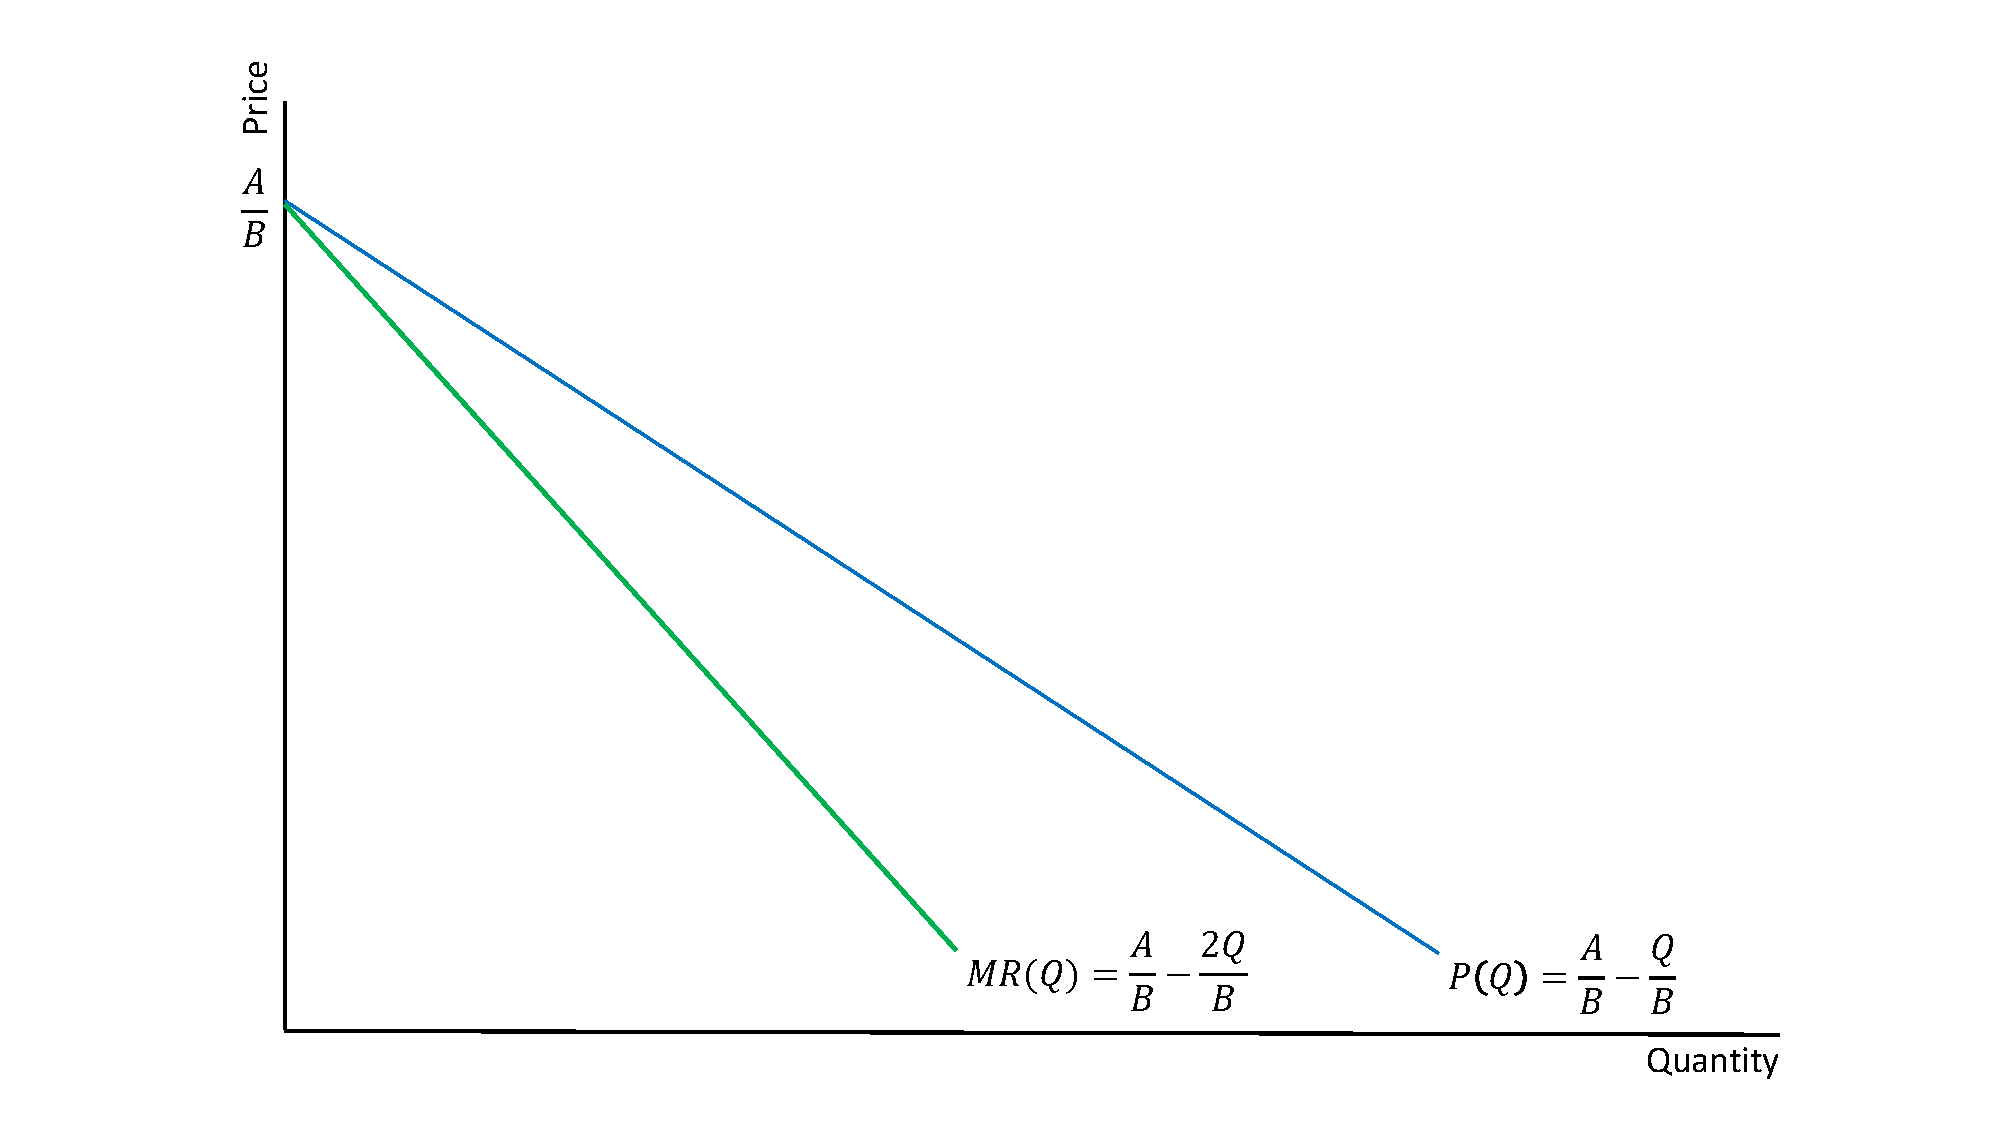
\includegraphics[scale=0.30]{SL2_1.pdf}

Notes:
	\begin{itemize}
		\item MR has double the slope of demand for linear demand curves
		\item MR always lies below demand (Why?)
	\end{itemize}

\end{frame}

\begin{frame}
	\frametitle{More Monopoly Terms}

\begin{itemize}
	\item \emph{Fixed Costs} $\equiv F$: A cost that does not depend on the level of output.
		\begin{itemize}
			\item Example: Rent
				\begin{itemize}
					\item Need to pay this for all $Q$ (even zero!)
					\item Fixed costs $\neq$ Sunk costs. 
				\end{itemize}
		\end{itemize}
	\item \emph{Variable Costs} $\equiv V(Q)$: Costs that depend on how much is produced
		\begin{itemize}
			\item Example: Labour costs.
		\end{itemize} 
	\item \emph{Total Cost} $\equiv TC(Q)$: How much must be spent to produce $Q$ units.
		\begin{itemize}
			\item $TC(Q)=V(Q)+F$
		\end{itemize}
	\item \emph{Average cost} $\equiv AC(Q)=\frac{TC(Q)}{Q}$: Total cost faced by the firm divided by the quantity produced \
	\item \emph{Marginal cost} $\equiv MC(Q)= (\frac{\partial TC}{\partial Q})$: Extra cost generated by producing an extra unit.

\end{itemize}

\end{frame}

\begin{frame}
\frametitle{Average and marginal cost}
Example: $TC(Q)=cQ+F$
	\begin{itemize}
		\item$ V(Q) =cQ$
	\end{itemize}
		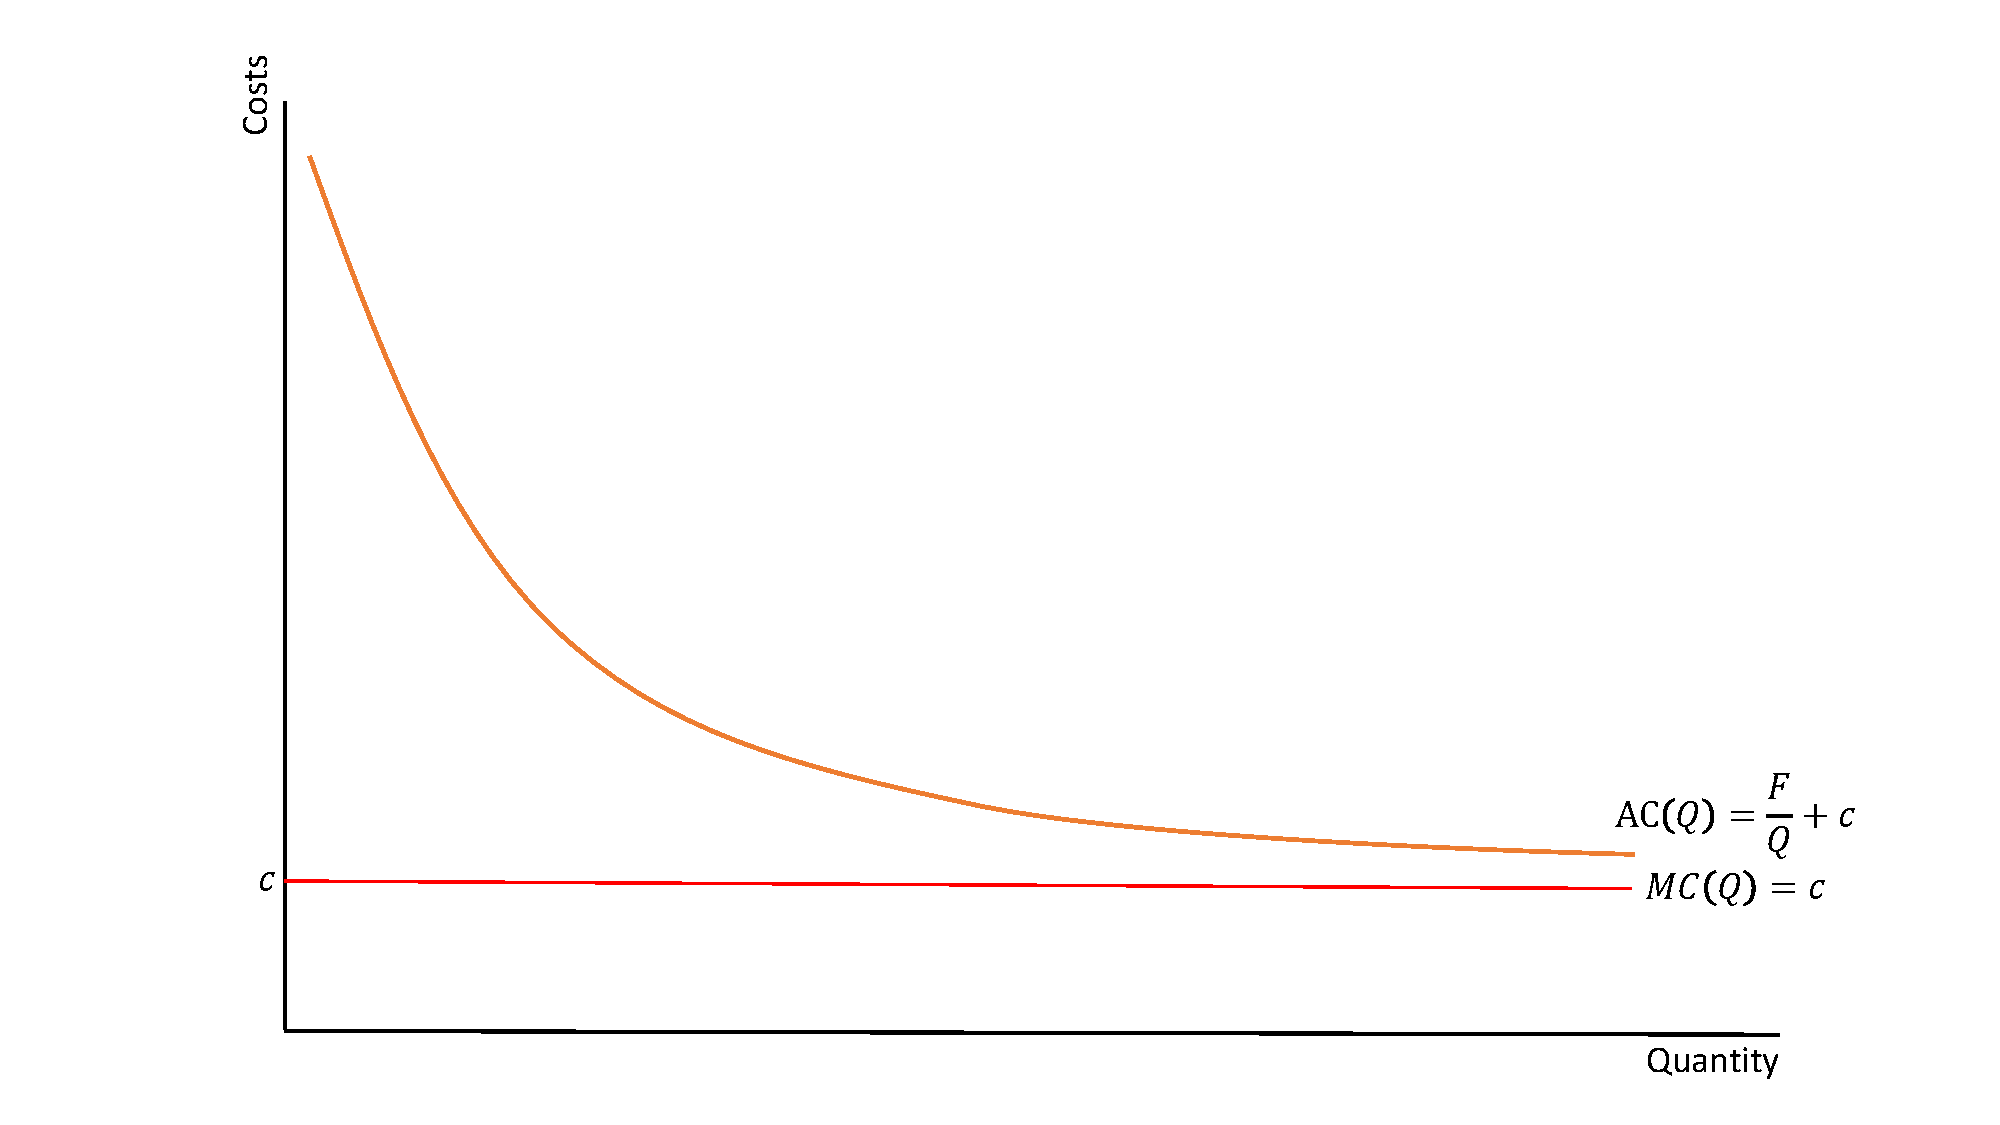
\includegraphics[scale=0.30]{SL2_2.pdf}

Note: Declining $AC\rightarrow$ Increasing returns to scale!

\end{frame}

\begin{frame}
	\frametitle{FOCs for Monopolist}

\noindent In general, the profit maximizing condition for a monopolist is:

\begin{equation}
MR(Q^*)=MC(Q*) \nonumber
\end{equation}

\begin{itemize}
	\item If $MR>MC$, monopolist earns greater profits by increasing production.
	\item If $MR<MC$, monopolist loses profits by increasing production.
\end{itemize}

\end{frame}

\begin{frame}
\frametitle{Profit maximization by the monopolist: Price}

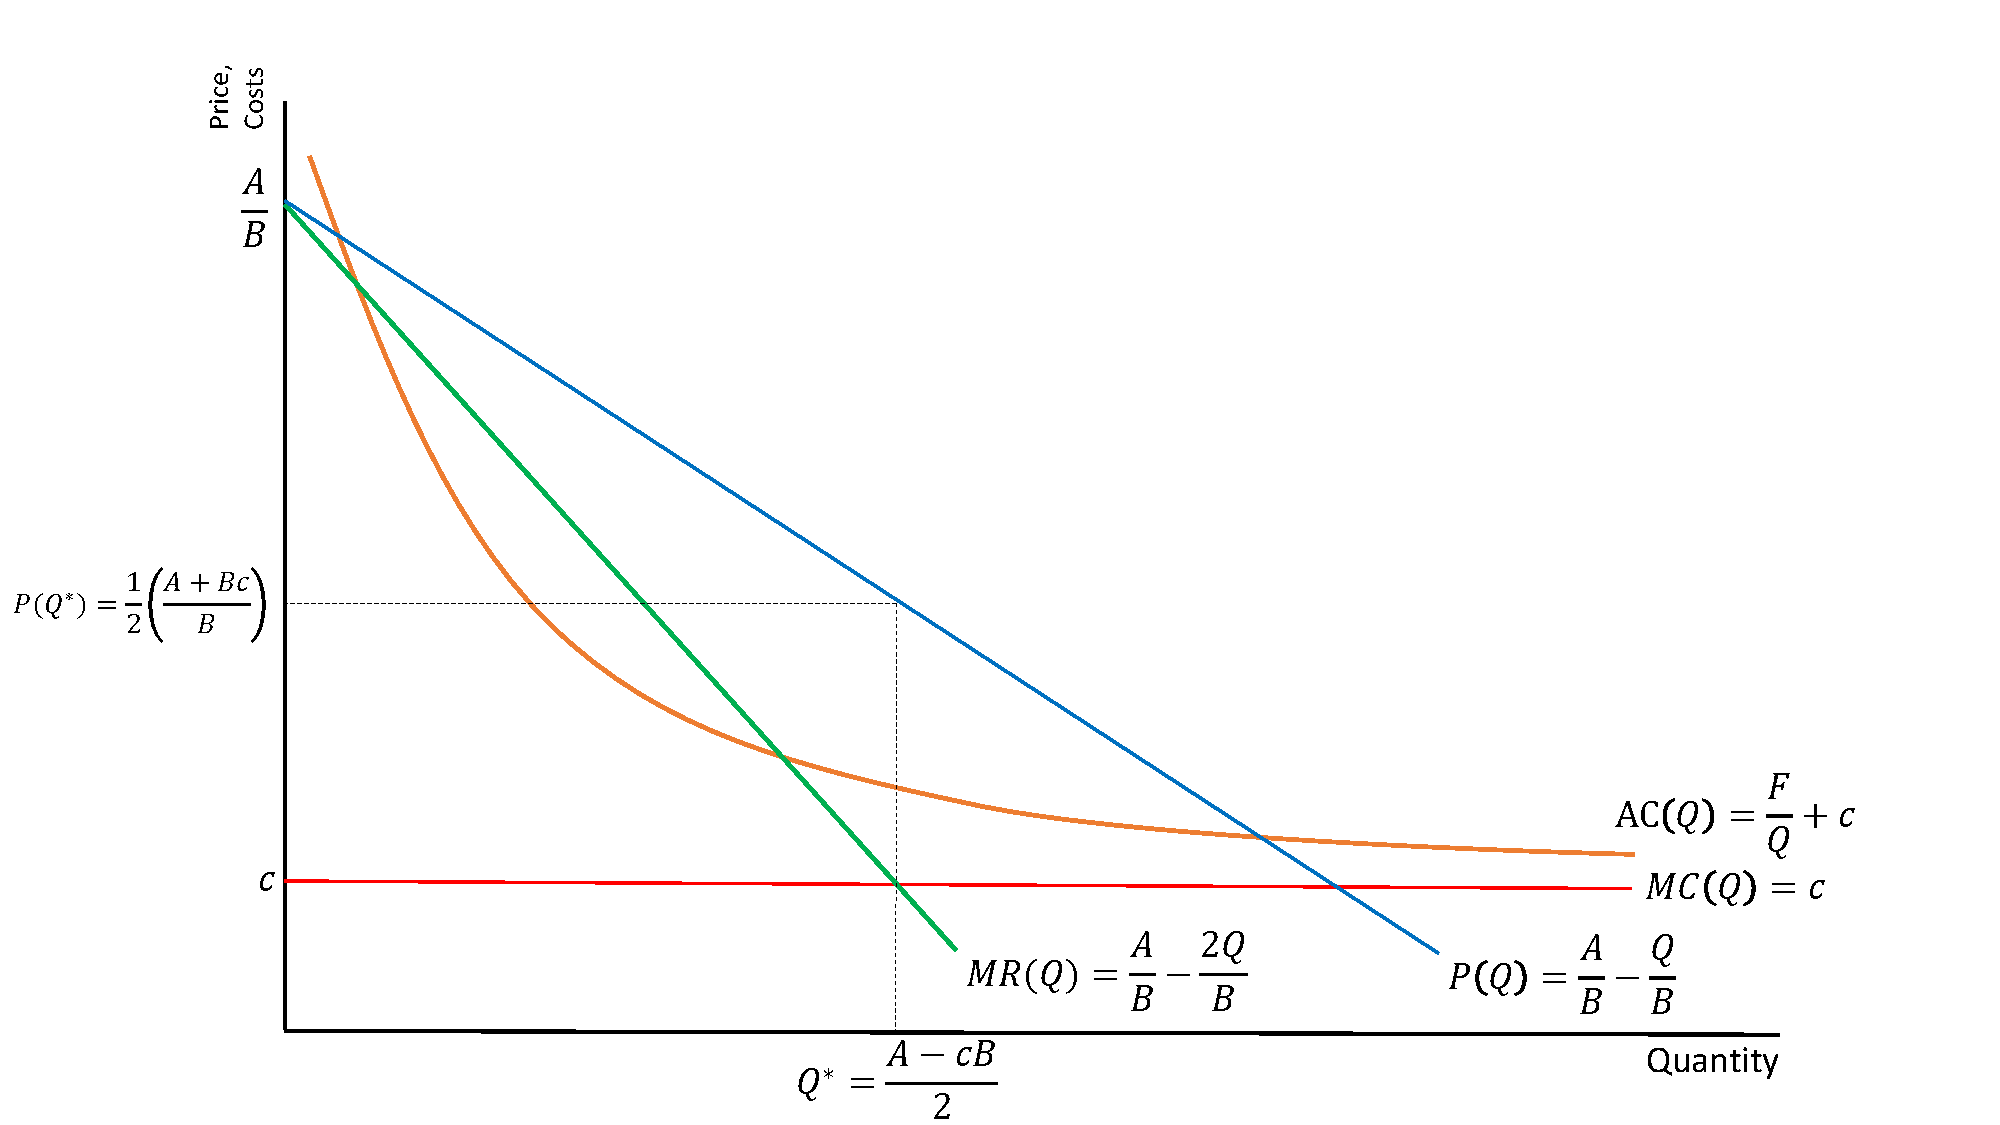
\includegraphics[scale=0.30]{SL2_3.pdf}
\end{frame}

\begin{frame}
	\frametitle{Profit maximization by the monopolist: Profits}
	
	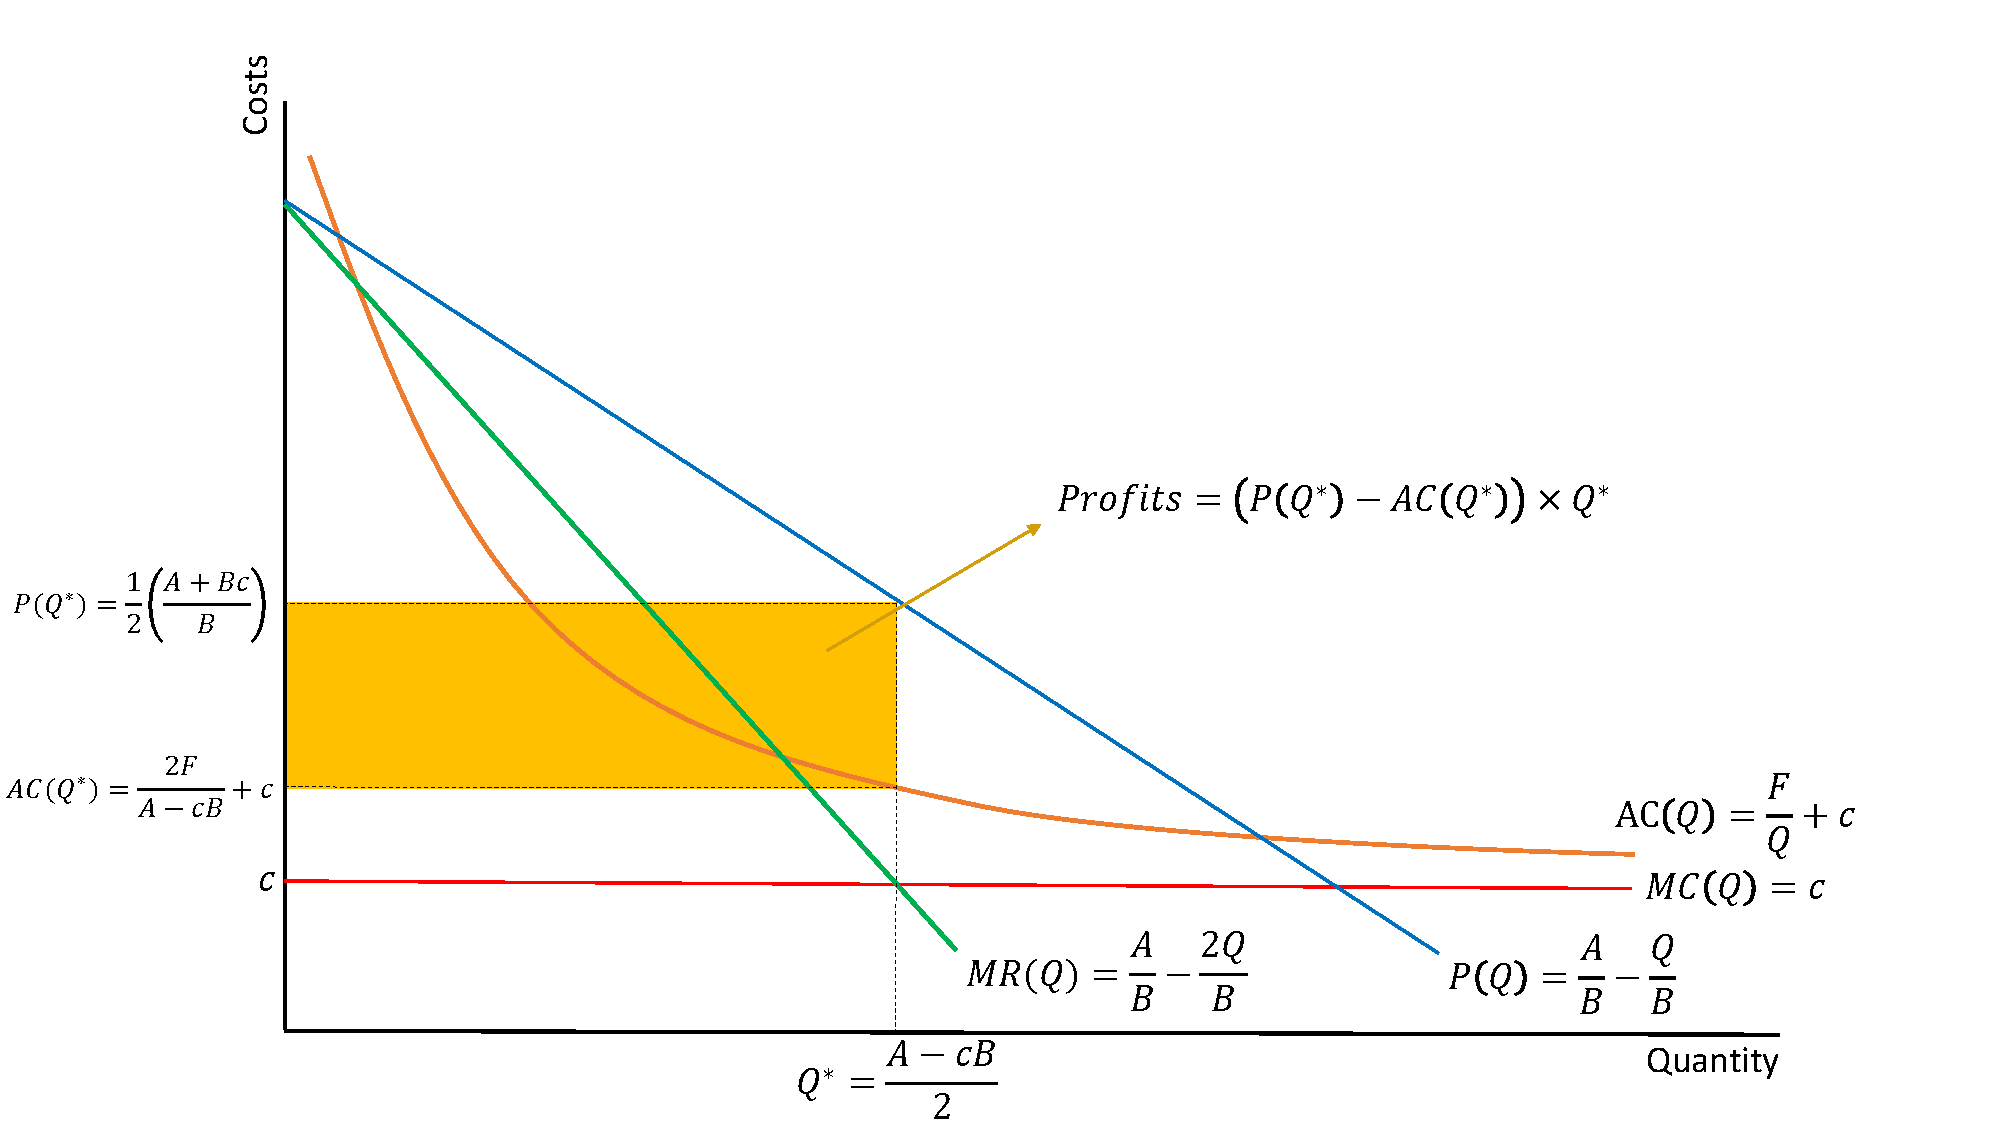
\includegraphics[scale=0.30]{SL2_4.pdf}
\end{frame}


\begin{frame}
	\frametitle{Basic Monopoly Results}
\begin{enumerate}
	\item Profit is maximized when marginal cost is equal to marginal revenue.
	\item Monopolists usually earn profits.
		\begin{itemize}
			\item Chose quantity so that $P>MC$
							\begin{itemize}
								\item Profits whenever $P>AC$
								\item Will hold as long as $F$ sufficiently small
							\end{itemize}
		\end{itemize}
\end{enumerate}

Let's now use the insights from our simple monopoly model to consider an environment with multiple firms.
\end{frame}

\subsection{Monopolistic Competition}

\begin{frame}
	\frametitle{Monopolistic Competition: Basic Setup}
	
Basically a model of oligopoly that works a lot like the monopoly model discussed before.
\begin{itemize}
	\item Key Assumptions:
		\begin{itemize}
			\item Firms differentiate their products 
				\begin{itemize}
					\item An increase in price will lower sales but not eliminate them. (Overcomes the Bertrand paradox)
					\item It is as if a firm is a monopolist for their own \emph{variety} of a product.
				\end{itemize}
			\item Rival firm prices affect the demand function faced by each firm.
				\begin{itemize}
					\item Competitive environment matters!
				\end{itemize} 
			\item Firms perceive their price as affecting own sales, but not rivals' price.
					\begin{itemize}
						\item Firms will take \emph{average prices} as given.
						\item More general oligopoly models relax this assumption.
					\end{itemize}
		\end{itemize}				
\end{itemize}



\end{frame}
\begin{frame}
\frametitle{Firm-level Demand}
Properties of the demand system:
\begin{itemize}
\item Firm $j$ sells more:
	\begin{itemize}
		\item The larger the size ($S$) of the market.
		\item The smaller the number of firms in the market ($n$)
		\item The lower its price ($p_j$)
		\item The higher the average price charged on the market ($\bar{p}\equiv\frac{1}{n}\sum^n_{k=1}p_k$)
	\end{itemize}
\end{itemize}
Example of a demand function satisfying these properties:
\[ q_j(p_j) = S \left[ \frac{1}{n} - b \left( p_j - \bar{p} \right) \right] \]


\end{frame}

\begin{frame}
	\frametitle{Firm-level Costs}
Assume a linear total cost function as in the monopoly case:
	\[ TC(q) = F + c q \]
		\begin{itemize}
			\item Variable costs $V(q)=cq$\vspace{2mm}
			\item Constant marginal costs 
			\begin{itemize}
				\item $MC(q) = \frac{\partial TC(q)}{\partial q} = c$ \vspace{3mm}
			\end{itemize}
			\item The fixed costs $F$ generate increasing returns to scale, i.e. falling average costs:
			\begin{itemize}
				\item $AC(q) = \frac{TC(q)}{q} = c + \frac{F}{q}$
			\end{itemize}
		\end{itemize}
\end{frame}

\begin{frame}

\frametitle{ Market equilibrium}

Note: we have assume that \emph{each} firms faces the same cost and demand function
	\begin{itemize}
		\item We will relax this assumption later.
	\end{itemize}

Consider a \emph{symmetric} equilibrium, i.e. $p_j=p \quad \forall j$
	\begin{itemize}
		\item While each firm \emph{could} set a different price, each firm will set the same price in an equilibrium because there are no differences between firms in efficiency nor how consumers value their output.
		\item Implies $q_j=q$ and $AC(q_j)=AC\quad \forall j$
	\end{itemize}


\end{frame}

\begin{frame}
	\frametitle{Recipe for solving the monopolistic competition model}
	
Determine equilibrium using 3 equations to pin down 3 unknowns: $\{n,p,AC\}$:
	\begin{enumerate}
		\item ``Average Cost Curve": Relationship between number of firms $(n)$ and average cost for each firm $(AC)$,
		\item ``Price Curve": Relationship between number of firms $(n)$ and price charged by each firm $(p)$,
		\item Close the model by assuming free entry and exit.
		\begin{itemize}
			\item Firms make zero profits, which means price $(p)$ must equal average cost $(AC)$
		\end{itemize}
	\end{enumerate}
\end{frame}

\begin{frame}
\frametitle{Deriving the average cost curve}
	\begin{itemize}
		\item When all firms charge the same price, $p = \bar{p} $, so:
		\begin{equation}
		q_j(p)=S \left[ \frac{1}{n} - b \left( p - \bar{p} \right) \right]=S \left[ \frac{1}{n} - 0 \right] = \frac{S}{n} = q \nonumber
		\end{equation}
		\item Substitute into average cost equation:
		\[ AC =   c + \frac{F}{q} = c + n \, \frac{F}{S} \]
		\item Equilibrium average cost increases with number of firms.
		\begin{itemize}
			\item With more firms for a given $S$, each firms sells a smaller quantity ($q$) and cannot exploit economies of scale as much.
		\end{itemize}
		\item Equilibrium average costs fall as the size of the market increases.
		\begin{itemize}
			\item If the market size increases for a given $n$, each firm sells a larger quantity ($q$) and can better exploit economies of scale.
		\end{itemize}
	\end{itemize}
\end{frame}


\begin{frame}
\frametitle{Average cost curve}
	\footnotesize
		\[ AC =   c + n \, \frac{F}{S} \]
	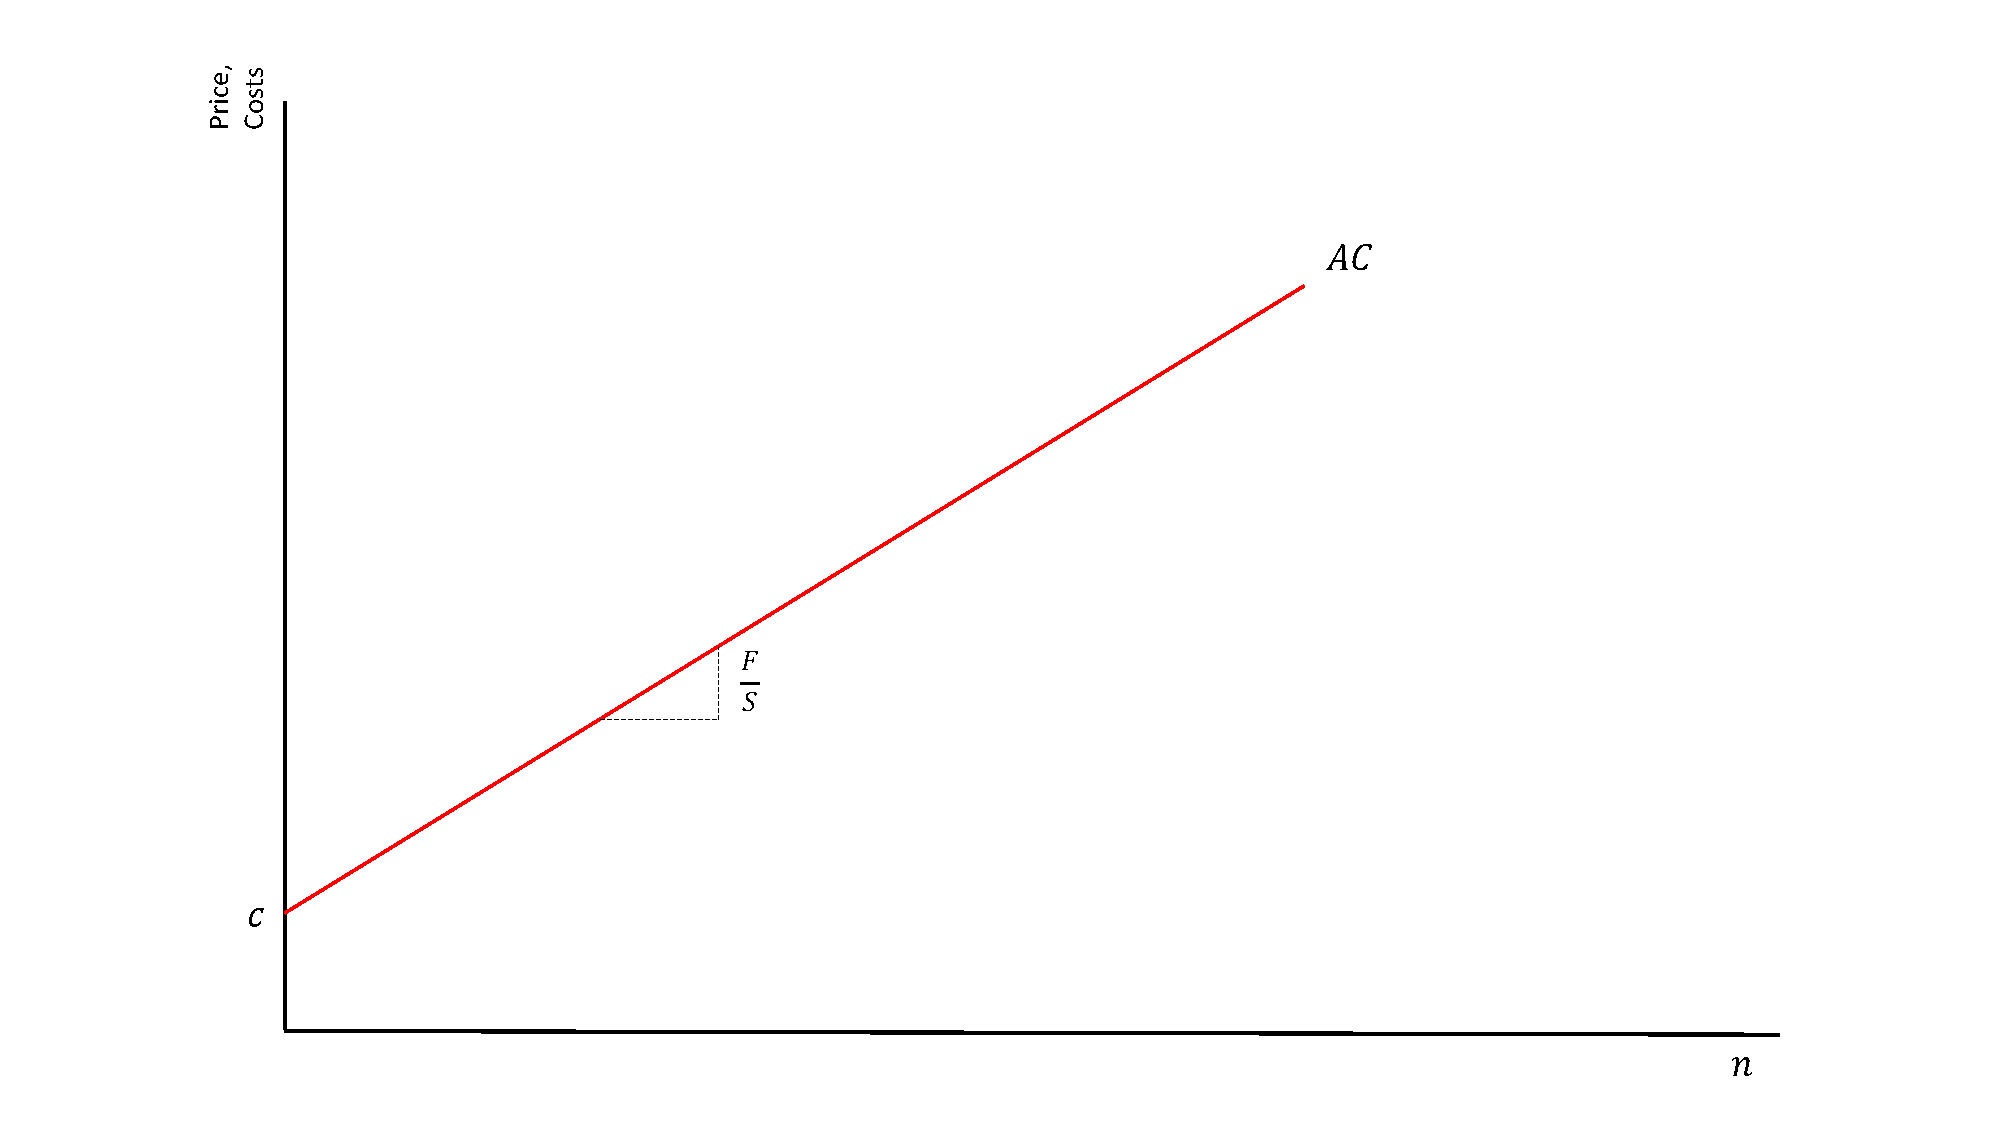
\includegraphics[scale=0.3]{SL2_5.pdf}
	
\end{frame}

\begin{frame}
	\frametitle{Deriving the price curve: Key condition}

Firms behave like a monopolist for the pricing of their particular variety.
		\begin{itemize}
			\item Profit maximization leads to the same first order condition:
			\begin{equation}
			MR_j=MC_j \nonumber
			\end{equation}
		\end{itemize}

We know marginal cost ($MC_j=c \quad \forall j$), so let's derive marginal revenue for a given firm:

\end{frame}

\begin{frame}
\frametitle{Deriving the price curve: Firm-level marginal review}
\footnotesize	

Recall from monopoly: Revenue $=R(q_j)=p(q_j)\times q_j$ $\rightarrow$

\begin{equation}
MR\equiv \frac{\partial R(q_j)}{\partial q_j}=p_j + \frac{\partial p(q_j)}{\partial q_j}\times q_j \nonumber
\end{equation}
\begin{itemize}
	\footnotesize
	\item Solve for the inverse demand function $p_j=p(q_j)$ using demand function $q_j=\left(\frac{S}{n} +Sb\bar{p} \right) -Sbp_j$:
	\begin{equation}
	p_j=p(q_j)=\left(\frac{1}{nb} + \bar{p} \right) -\frac{q_j}{Sb} \nonumber
	\end{equation}
	\item Partially differentiate inverse demand to obtain $\frac{\partial p(q_j)}{\partial q_j}$ (Holding $\bar{p}$ fixed!)
	\begin{equation}
	\frac{\partial p(q_j)}{\partial q_j}= \frac{-1}{Sb} \nonumber
	\end{equation}
	\item Marginal revenue given by:
	\begin{equation}
	MR_j=p_j-\frac{q_j}{Sb} \nonumber
	\end{equation}
\end{itemize}
\end{frame}

\begin{frame}
	\frametitle{Deriving the price curve}

Rearrange profit maximizing condition  $MR_j=MC_j$
\begin{equation}
p_j-\frac{q_j}{Sb}=c \nonumber
\end{equation} 
\begin{equation}
p_j=c + \frac{q_j}{Sb} \nonumber
\end{equation} 
Recall that we are considering a symmetric equilibrium, so $q_j=q=\frac{S}{n}$ and $p_j = p \quad \forall j$
\begin{equation}
p=c + \frac{1}{bn} \nonumber
\end{equation} 
	\begin{itemize}
		\item Note: DO NOT impose symmetry before deriving firm level marginal revenue (Why?)
	\end{itemize}
	


\end{frame}

\begin{frame}
	\footnotesize
\begin{equation}
p=c + \frac{1}{bn} \nonumber
\end{equation} 
	\frametitle{Price curve}
	\begin{center}
			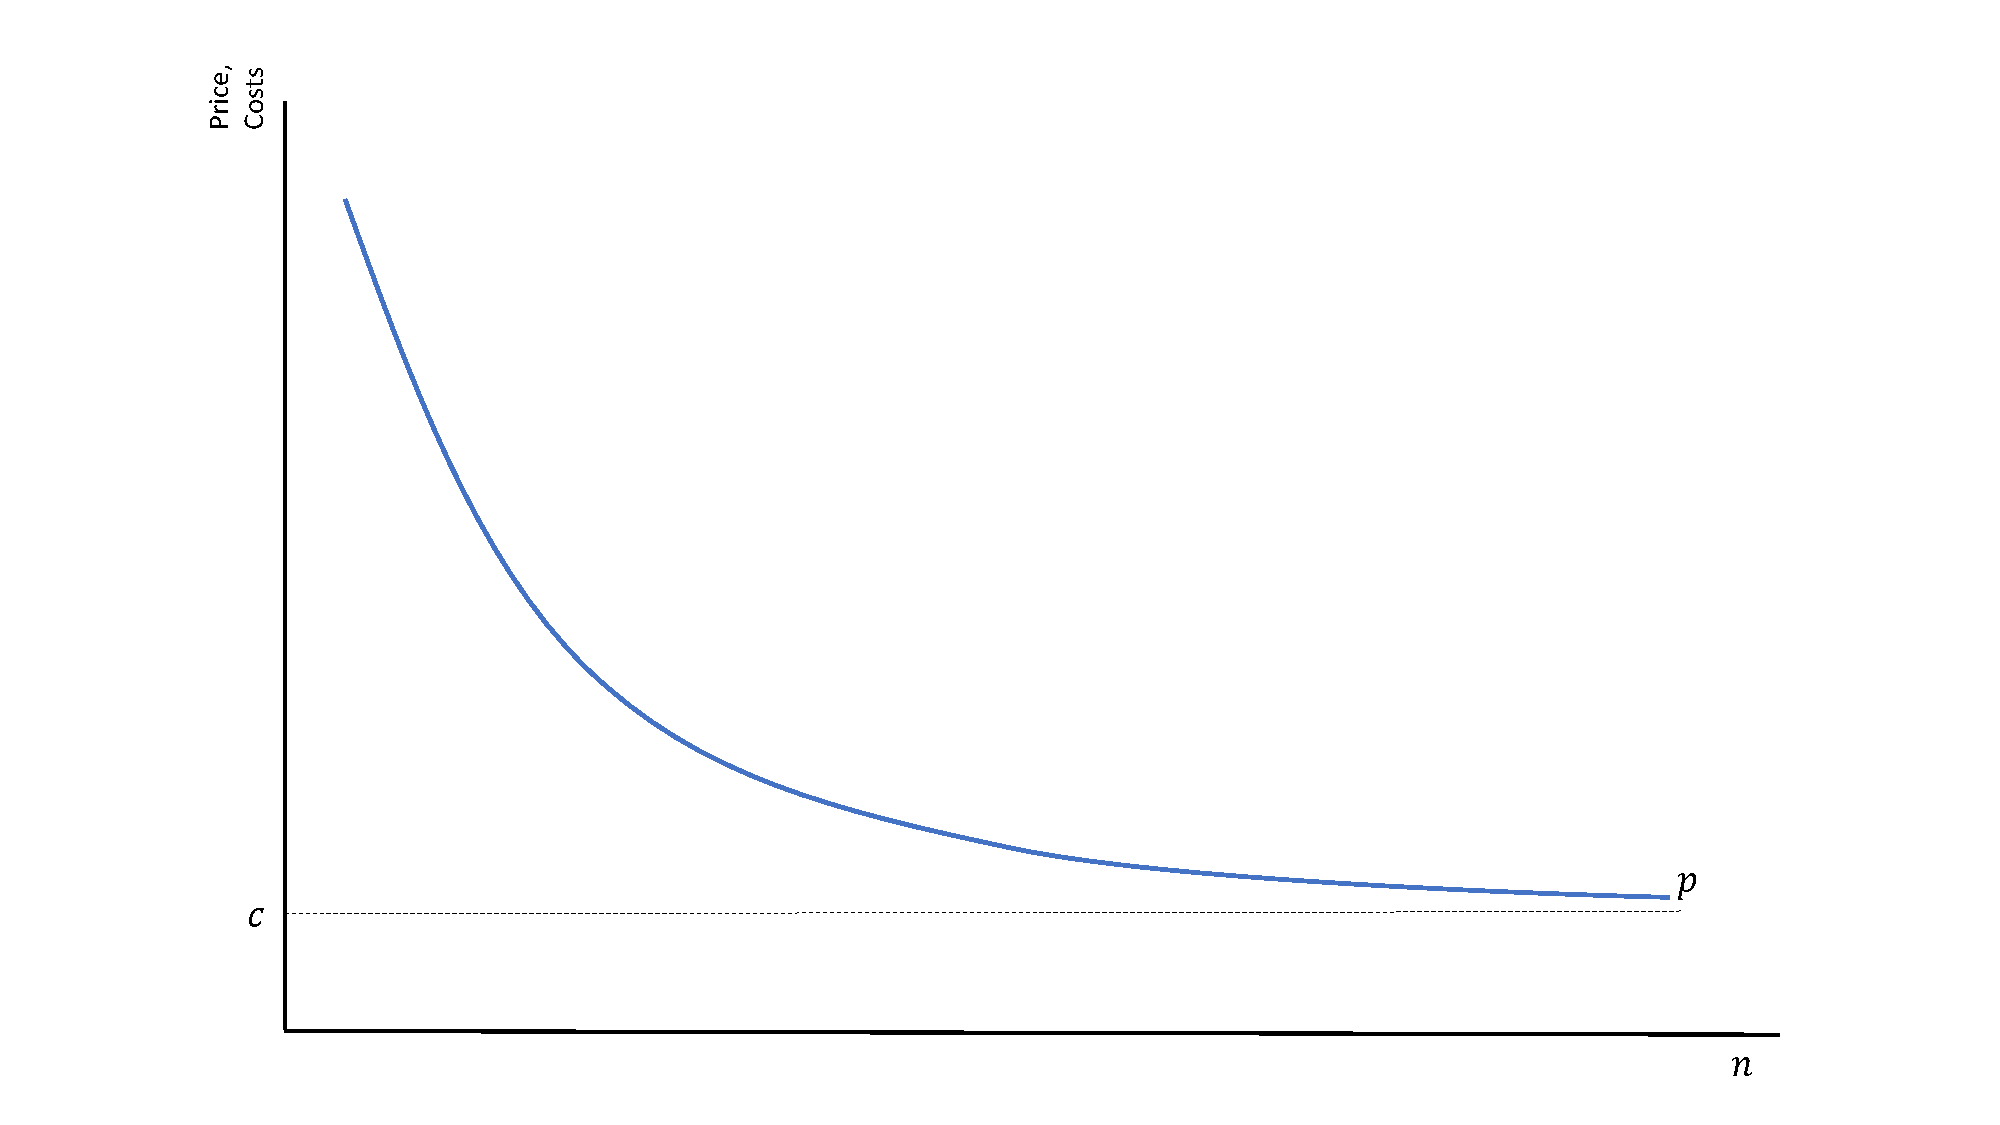
\includegraphics[scale=0.25]{SL2_6.pdf}
	\end{center}

	\begin{itemize}
		\footnotesize
		\item $p>MC$ due to the \emph{markup} $\equiv \mu = \frac{1}{bn}$
		\item Markups fall as more firms enter (more competition $\rightarrow$ less market power), and as price sensitivity rises $b$.

	\end{itemize}
	
\end{frame}

\begin{frame}
\frametitle{Closing the model}
We assume free entry and exit.
	\begin{itemize}
		\item With identical firms, this means that firms enter (exit) until everyone earns zero profits
		\begin{equation}
		p = AC \nonumber
		\end{equation}
		\item From our derivation of the average cost and price curves, we also know that in equilibrium:
		$$AC=c+n\frac{F}{S}$$
		$$p=c+\frac{1}{bn}$$
		
		\item Intersection of average cost and price curves (where $p=AC$) determines the equilibrium number of firms
	\end{itemize}

	
\end{frame}

\begin{frame}
\frametitle{Equilibrium}
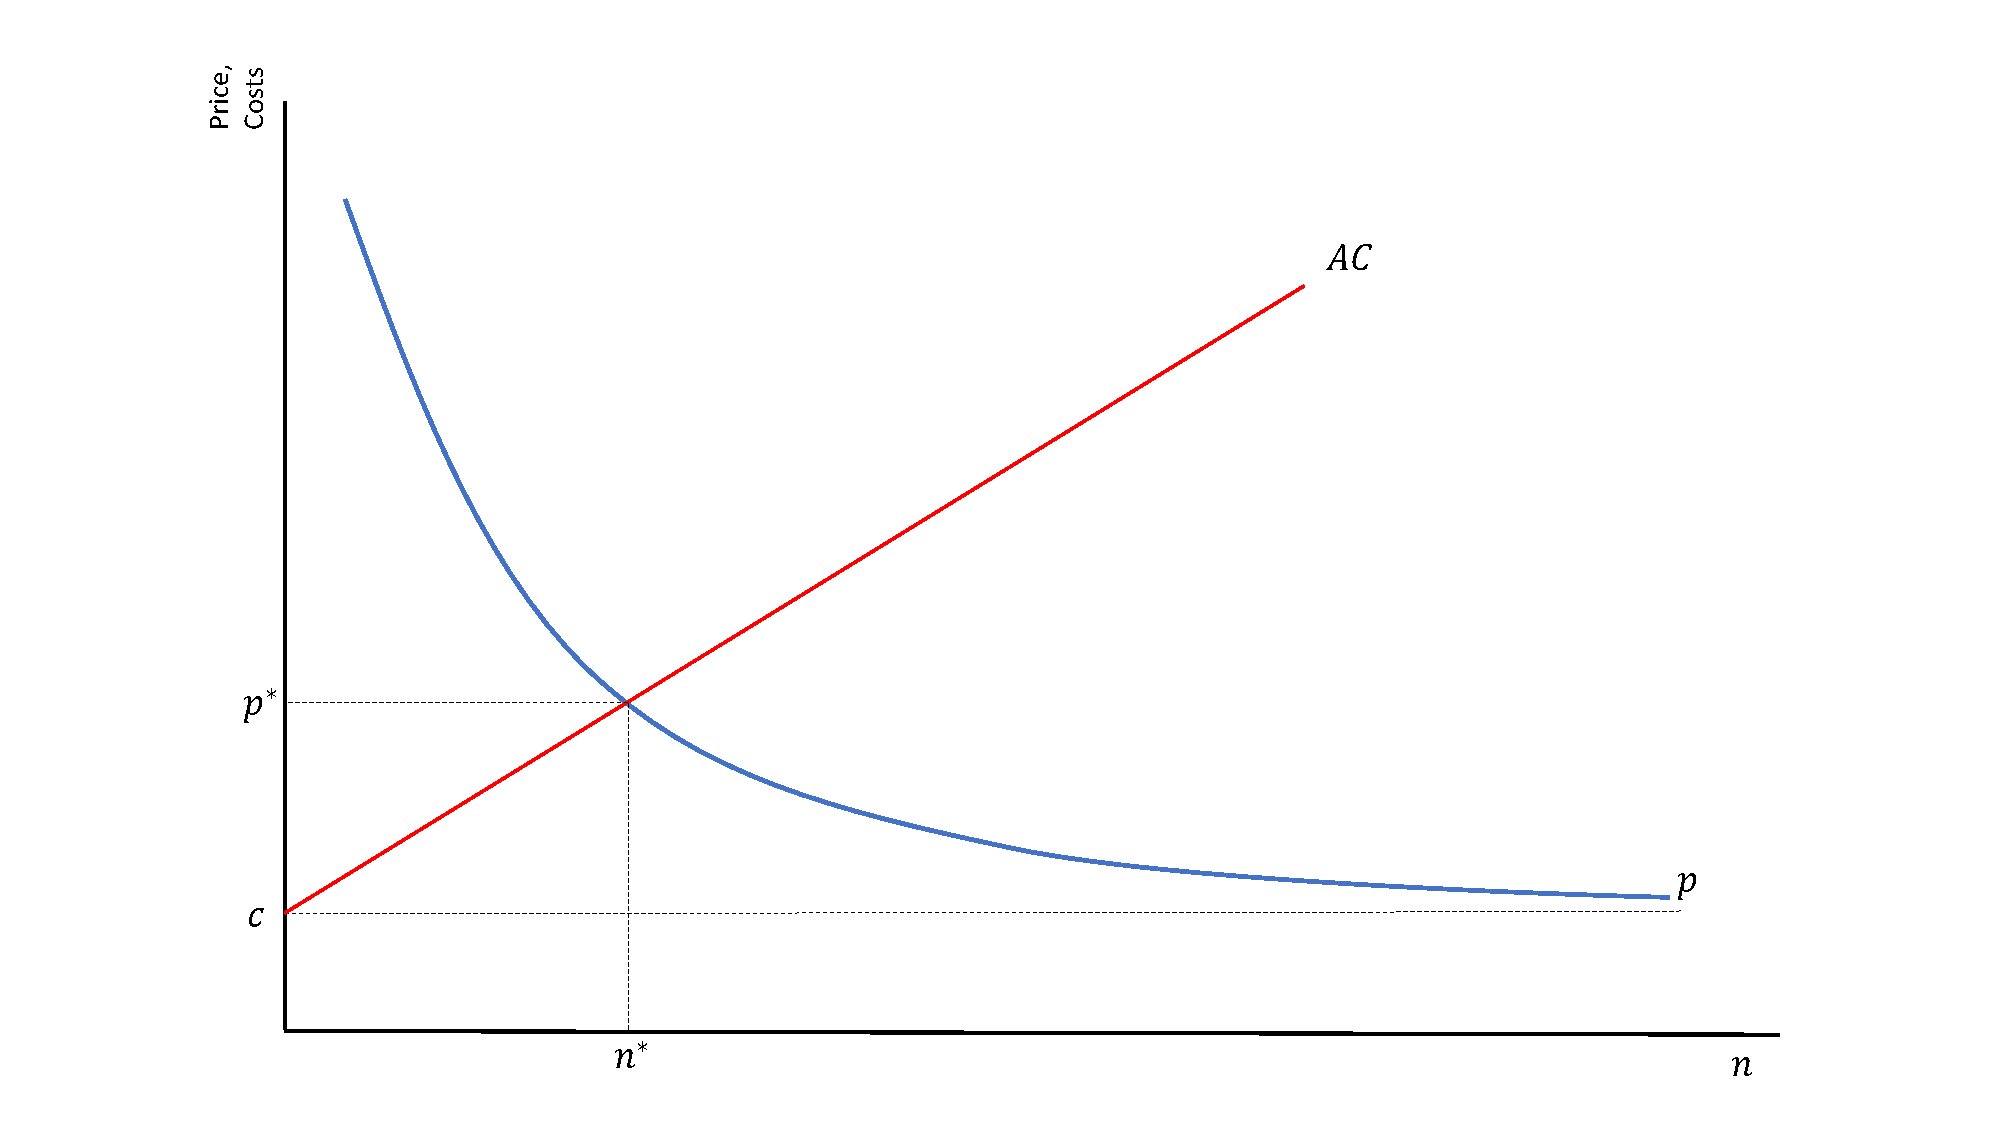
\includegraphics[scale=0.3]{SL2_7.pdf}

\scriptsize
Or analytically:
	\begin{equation}
	n^* =\left(\frac{S}{Fb}\right)^{1/2} \nonumber
	p^*=c + \left(\frac{F}{bS}\right)^{1/2}
	\end{equation}


\end{frame}

\begin{frame}
\frametitle{Monopolistic Competition and Trade}
Trade can be seen as an increase in market size (Krugman 1979)
\begin{itemize}
	\item $\uparrow S$
	\item Recall:
				$$AC=c+n\frac{F}{S}$$
				$$p=c+\frac{1}{bn}$$
	\item Average cost curve \emph{rotates} downwards, price curve remains constant
\end{itemize}

\end{frame}

\begin{frame}
	\frametitle{Monopolistic Competition and Trade}
	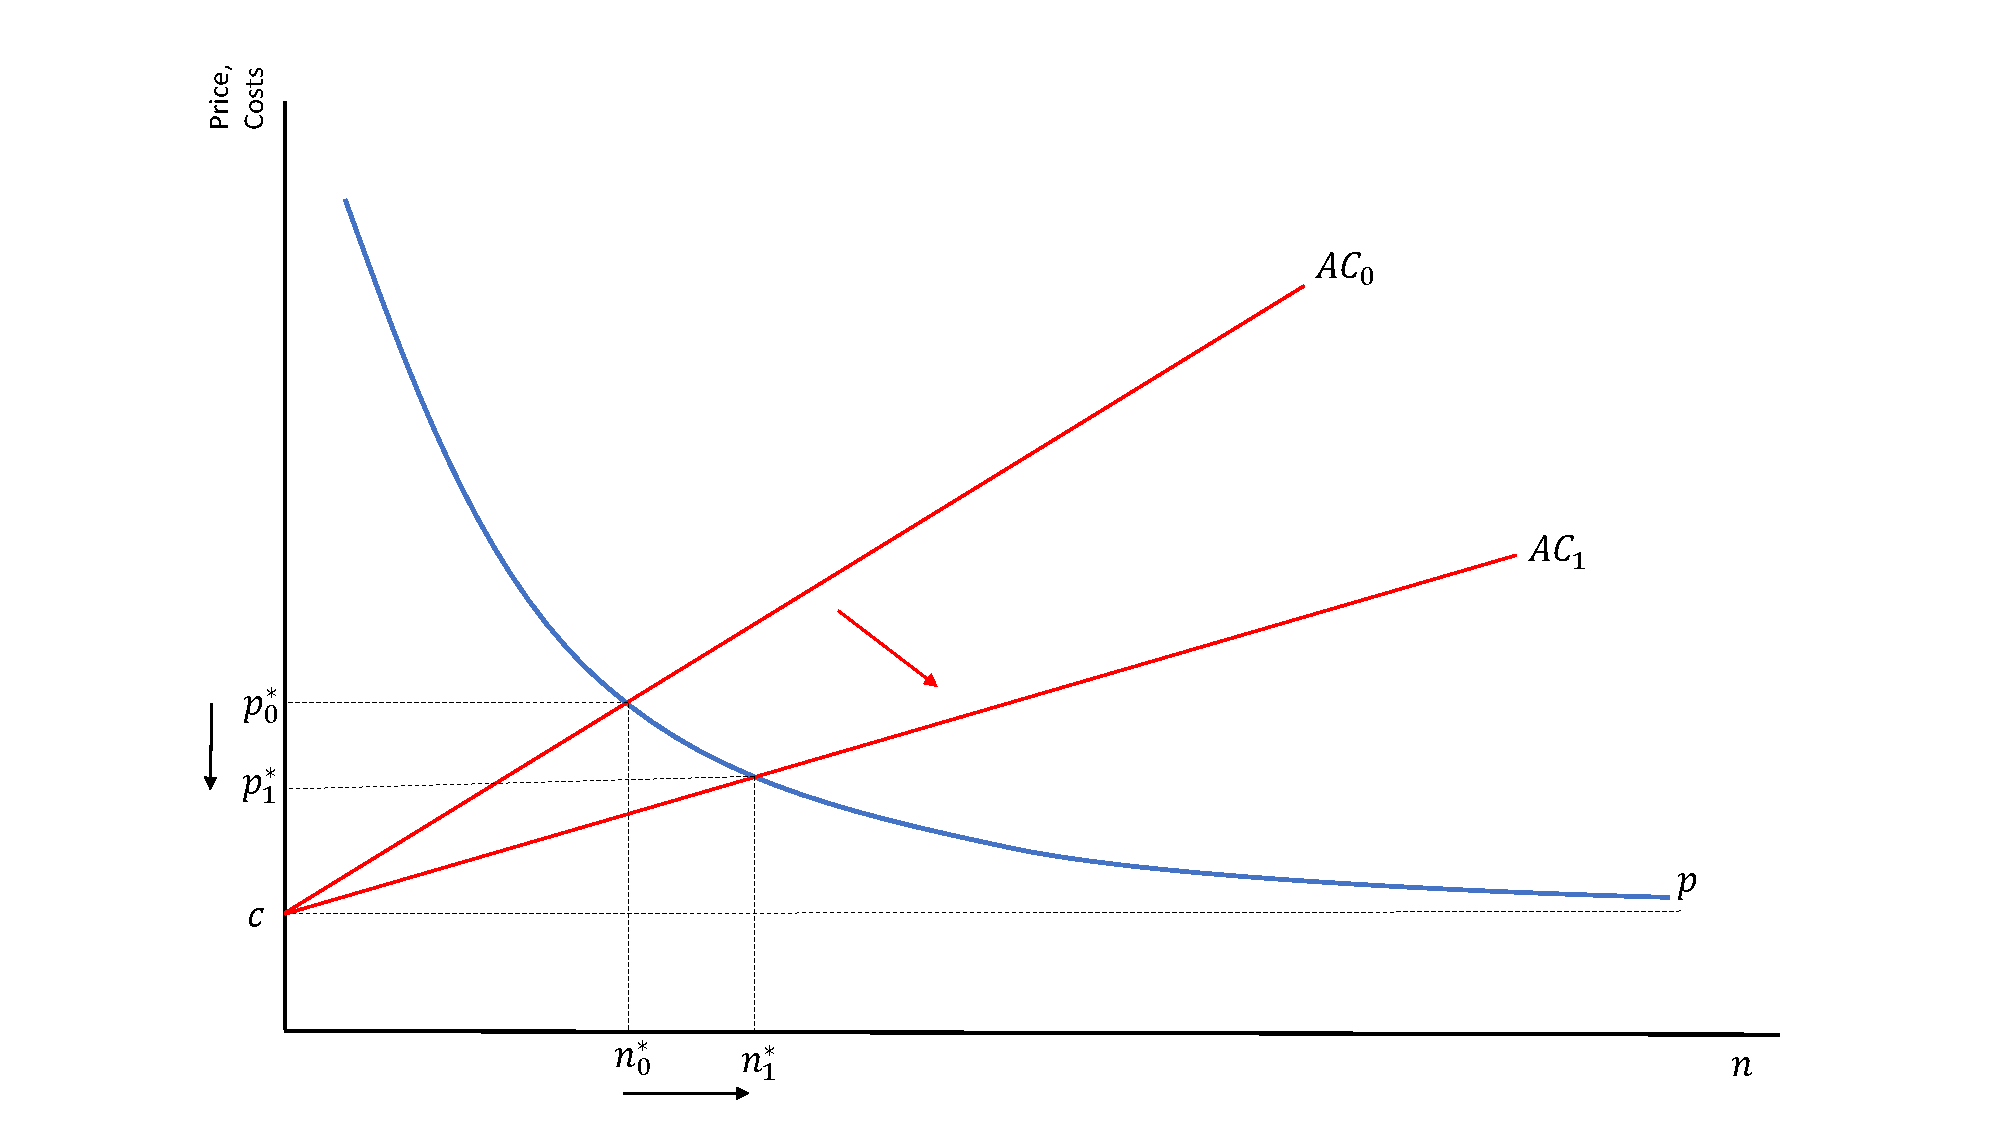
\includegraphics[scale=0.32]{SL2_8.pdf}
\end{frame}


\begin{frame}
	\frametitle{Gains from trade with monopolistic competition}
\begin{itemize}
	\item When two countries open up to trade, the integrated market sustains more varieties of goods than each of the two markets did alone.
	\begin{itemize}
		\item $\uparrow n$: Consumers gain from more varieties/firms.
	\end{itemize}
	\item Because under free trade each firm produces at a larger scale, it can exploit economies of scale further, cutting costs.
		\begin{itemize}
			\item Recall $q=\frac{S}{n}$
							\begin{itemize}
								\item While both $S$ and $n$ rise, can show that $\uparrow S > \uparrow n$ (Problem Set 4)
							\end{itemize}
		\end{itemize}

	\item Consumer gain from lower prices.
			\begin{itemize}
			\item Recall that markups are given by: $\mu=\frac{1}{bn}$
			\item $\uparrow n$, increased competition, firms decrease their markups, and prices fall.
			\item So called ``Pro-competitive" gains from trade. 
			\end{itemize}
\end{itemize}

\end{frame}

\begin{frame}
	\frametitle{Market size, trade integration, and competition}
We have just considered opening up to trade as an increase in market size, and showed that this increases the number of firms selling to a \emph{particular country} in equilibrium.
	\begin{itemize}
		\item Note that there will generally be more firms operating \emph{across} the two countries before integration.
			\begin{itemize}
				\item While varieties available to each consumer increases, increased competition causes some firms to exit the market.
				\item We tend to see effects of this sort in practice:
					\begin{itemize}
						\item Following NAFTA, General Motors cut in half the number of car models produced in Canada. 
					\end{itemize}
			\end{itemize}
	\end{itemize}
\end{frame}

\begin{frame}
	\frametitle{Exit-Effects Following Trade LIberalization}	

Consider two completely identical countries:
	\begin{itemize}
		\item Autarky number of firms in each country:
		\begin{itemize}
			\item $n^A=\left(\frac{S}{Fb}\right)^{1/2}$
			\item Overall number of firms $2n^A=2n^A=\left(\frac{S}{Fb}\right)^{1/2}$
		\end{itemize}
		\item Total number of firms in the free-trade \emph{integrated} equilibrium
			\begin{itemize}
			\item $n^T=\left(\frac{2S}{Fb}\right)^{1/2}$
			\end{itemize}
		\item Note that since $\sqrt{2}<2$
			\scriptsize
			\begin{equation}
			n^T = \left(\frac{2S}{Fb}\right)^{1/2} = \sqrt{2}\left(\frac{S}{Fb}\right)^{1/2} < 2\left(\frac{S}{Fb}\right)^{1/2}  = 2n^A \nonumber
			\end{equation}
			\normalsize
		\item Clearly some firms will have to exit the market following trade-liberalization!
			\begin{itemize}
				\item However, since $n^A<n^T$, still gains from trade, \emph{even though countries are identical}
			\end{itemize}
	\end{itemize}
	
\end{frame}

\begin{frame}
	\frametitle{Exit-Effects Following Trade Liberalization}
While some firms will exit the market following trade integration, model makes no predictions as to \emph{who} will exit the market.
	\begin{itemize}
		\item Empirical literature has generally found that \emph{less productive} firms are most likely to exit the market following trade liberalization (E.g. Pavcnik 2002).
		\item To make sense of these facts, we need a model that accounts for \emph{firm heterogeneity}
			\begin{itemize}
				\item Next class!
			\end{itemize}
	\end{itemize}
\end{frame}

\begin{frame}
	\frametitle{What have we learned today?}
	\begin{itemize}
		\item Other Trade Policy Instruments:	
			\begin{itemize}
				\item Export subsidies hurt large and small open economies. Quotas and VERs hurt small open economies.
			\end{itemize}
		\item Politics:
			\begin{itemize}
				\item Trade barriers may be due to distributional concerns, politically motivated concerns, collective action problems, or terms of trade considerations
			\end{itemize}
		\item Firms and the Global Economy
			\begin{itemize}
				\item Models of trade with increasing returns to scale and market power needed to understand ``intra-industry" trade.
				\item Pro-competitive gains from trade and gains from variety.
			\end{itemize}
	\end{itemize}
\end{frame}

\begin{frame}
	\frametitle{Extra References}
	\scriptsize
Baldwin, Robert and Christopher Magee (2000) ``Is trade policy for sale? Congressional voting on recent trade bills." \emph{Public Choice} 105: 79-101. \\ \vspace{2mm}
Broda, Christian, Nuno Limao and David Weinstein (2008) ``Optimal Tariffs and Market Power." \emph{American Economic Review} 98: 2032-2065. \\ \vspace{2mm}
Dhingra, Swati (2014) ``Reconciling observed tariffs and the median voter model." \emph{Working paper} \\ \vspace{2mm}
Downs, Anthony (1957) \emph{An Economic Theory of Democracy} (Washington, D.C.: Brookings Institution) \\ \vspace{2mm}
Dutt, Pushan, and Devashish Mitra (2002) ``Endogenous trade policy through majority voting: an empirical investigation." \emph{Journal of International Economics}, 58: 107-133. \\ \vspace{2mm}
Olson, Mancur (1965)  \emph{The Logic of Collective Action} (Cambridge: Harvard University Press) \\  \vspace{2mm}
Pavcnik, Nina (2002) ``Trade Liberalization, Exit, and Productivity Improvements: Evidence from Chilean Plants" \emph{Review of Economic Studies} 69: 245-276.
\end{frame}

\end{document}